\renewcommand{\thefigure}{S\arabic{figure}}

\clearpage
\begin{figure}[ht]
    \begin{subfigure}[t]{.5\textwidth}
        \caption{}
        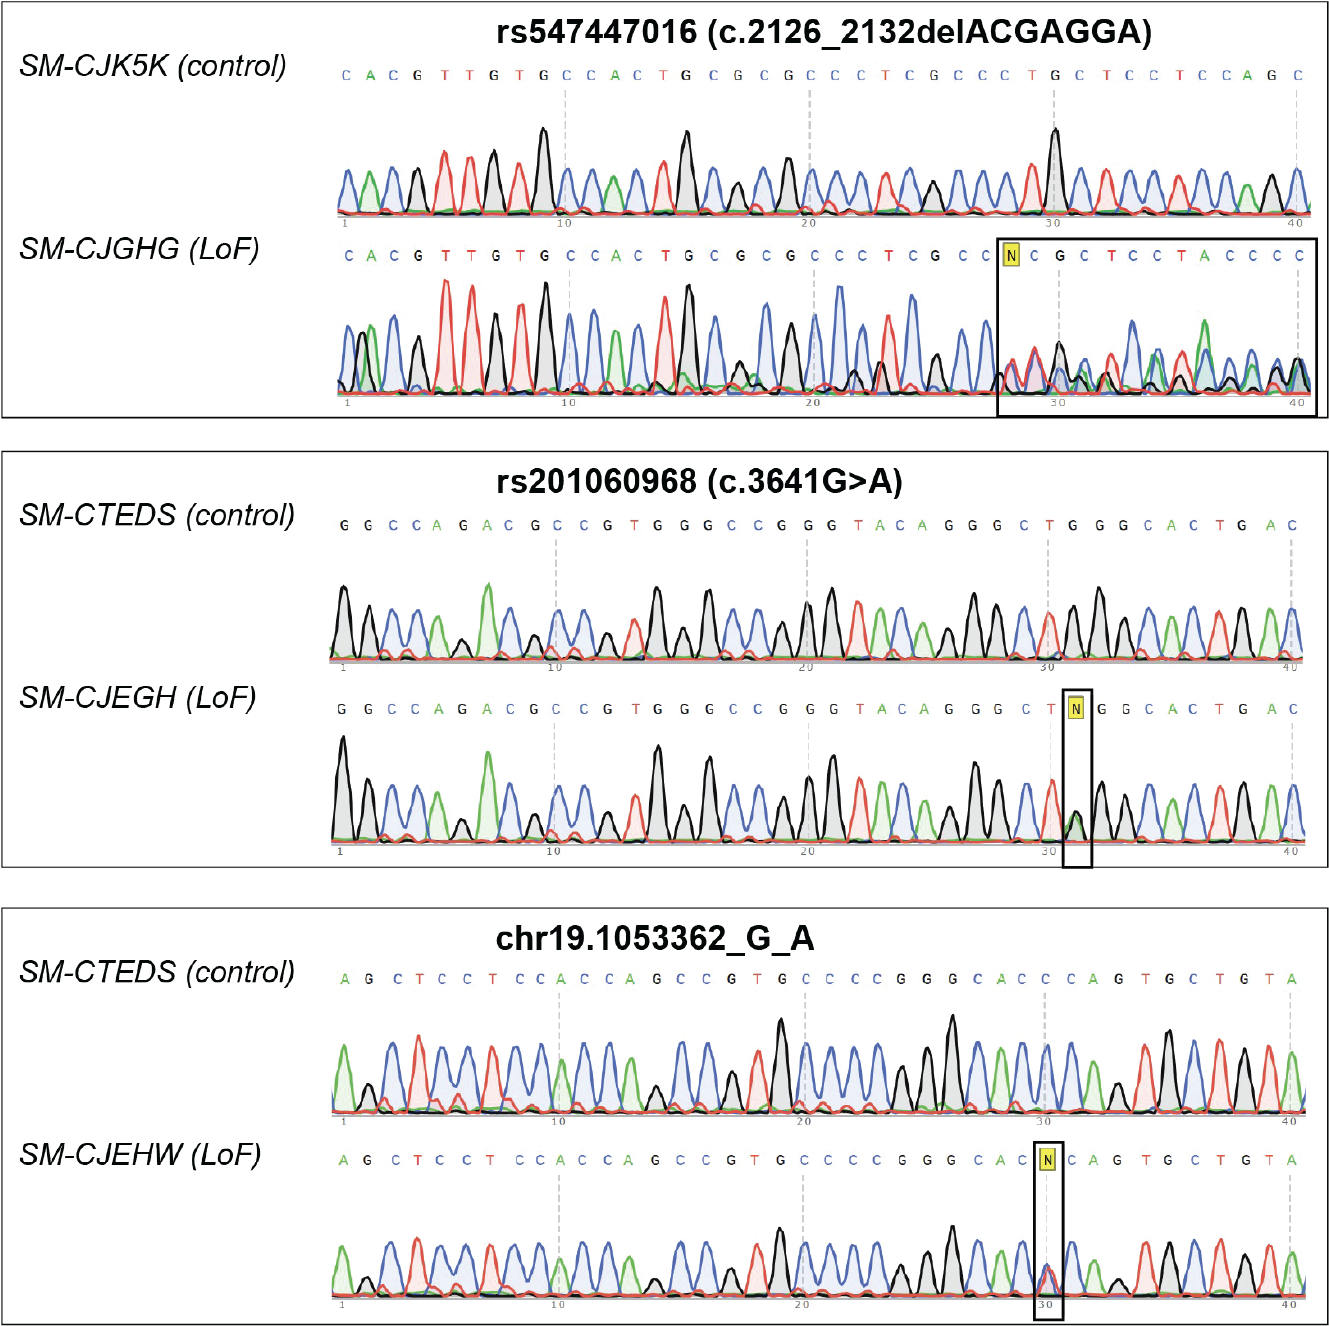
\includegraphics[width=\textwidth]{./extended_plots/sanger_seq.png}        
    \end{subfigure}  
    \begin{subfigure}[t]{.5\textwidth}
        \begin{subfigure}[t]{\textwidth}
            \caption{}
            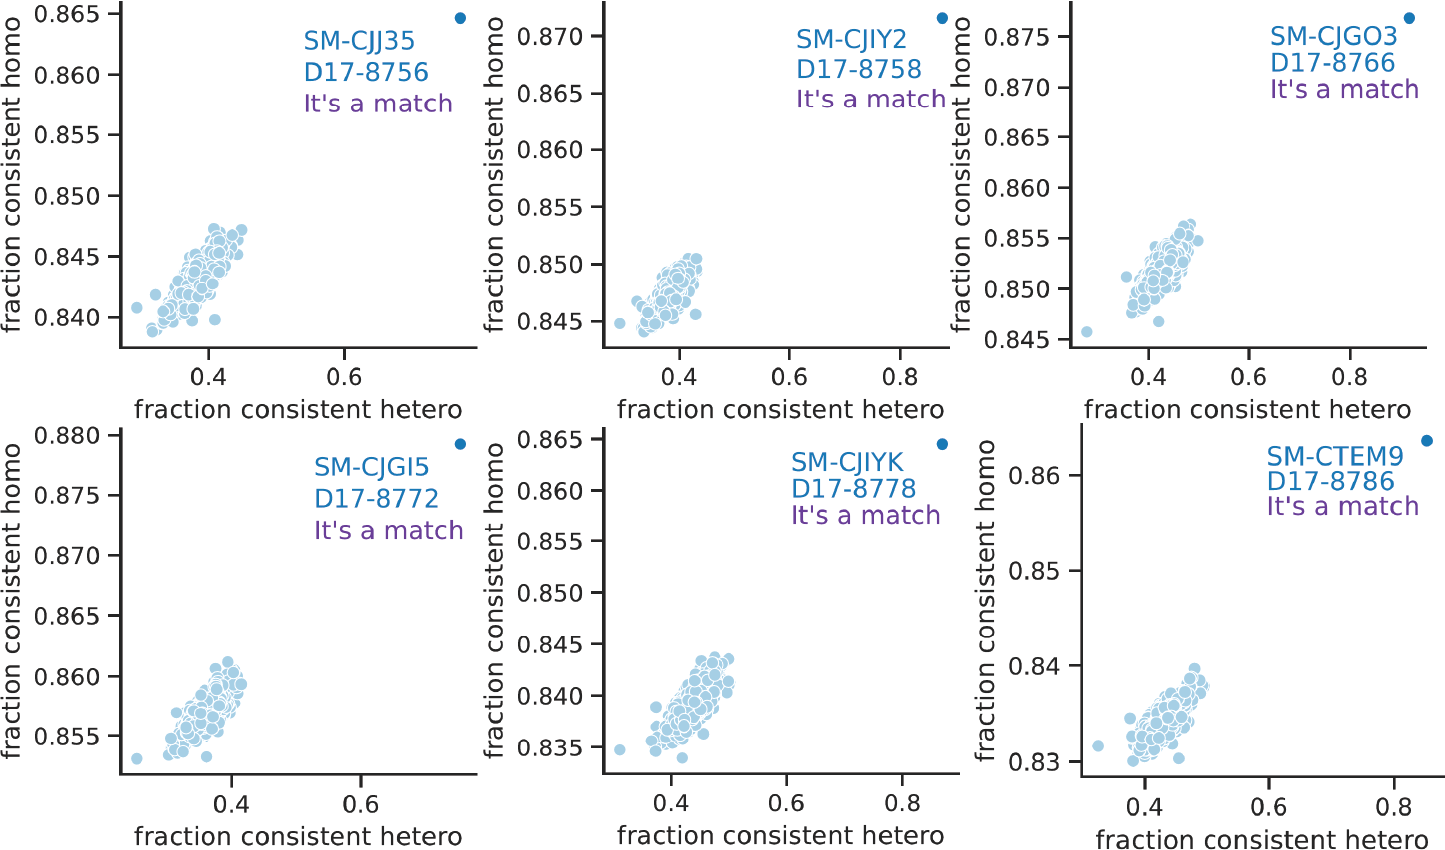
\includegraphics[width=\textwidth]{./extended_plots/sample_swap.png}        
        \end{subfigure}  
        \begin{subfigure}[t]{\textwidth}
            \caption{}
            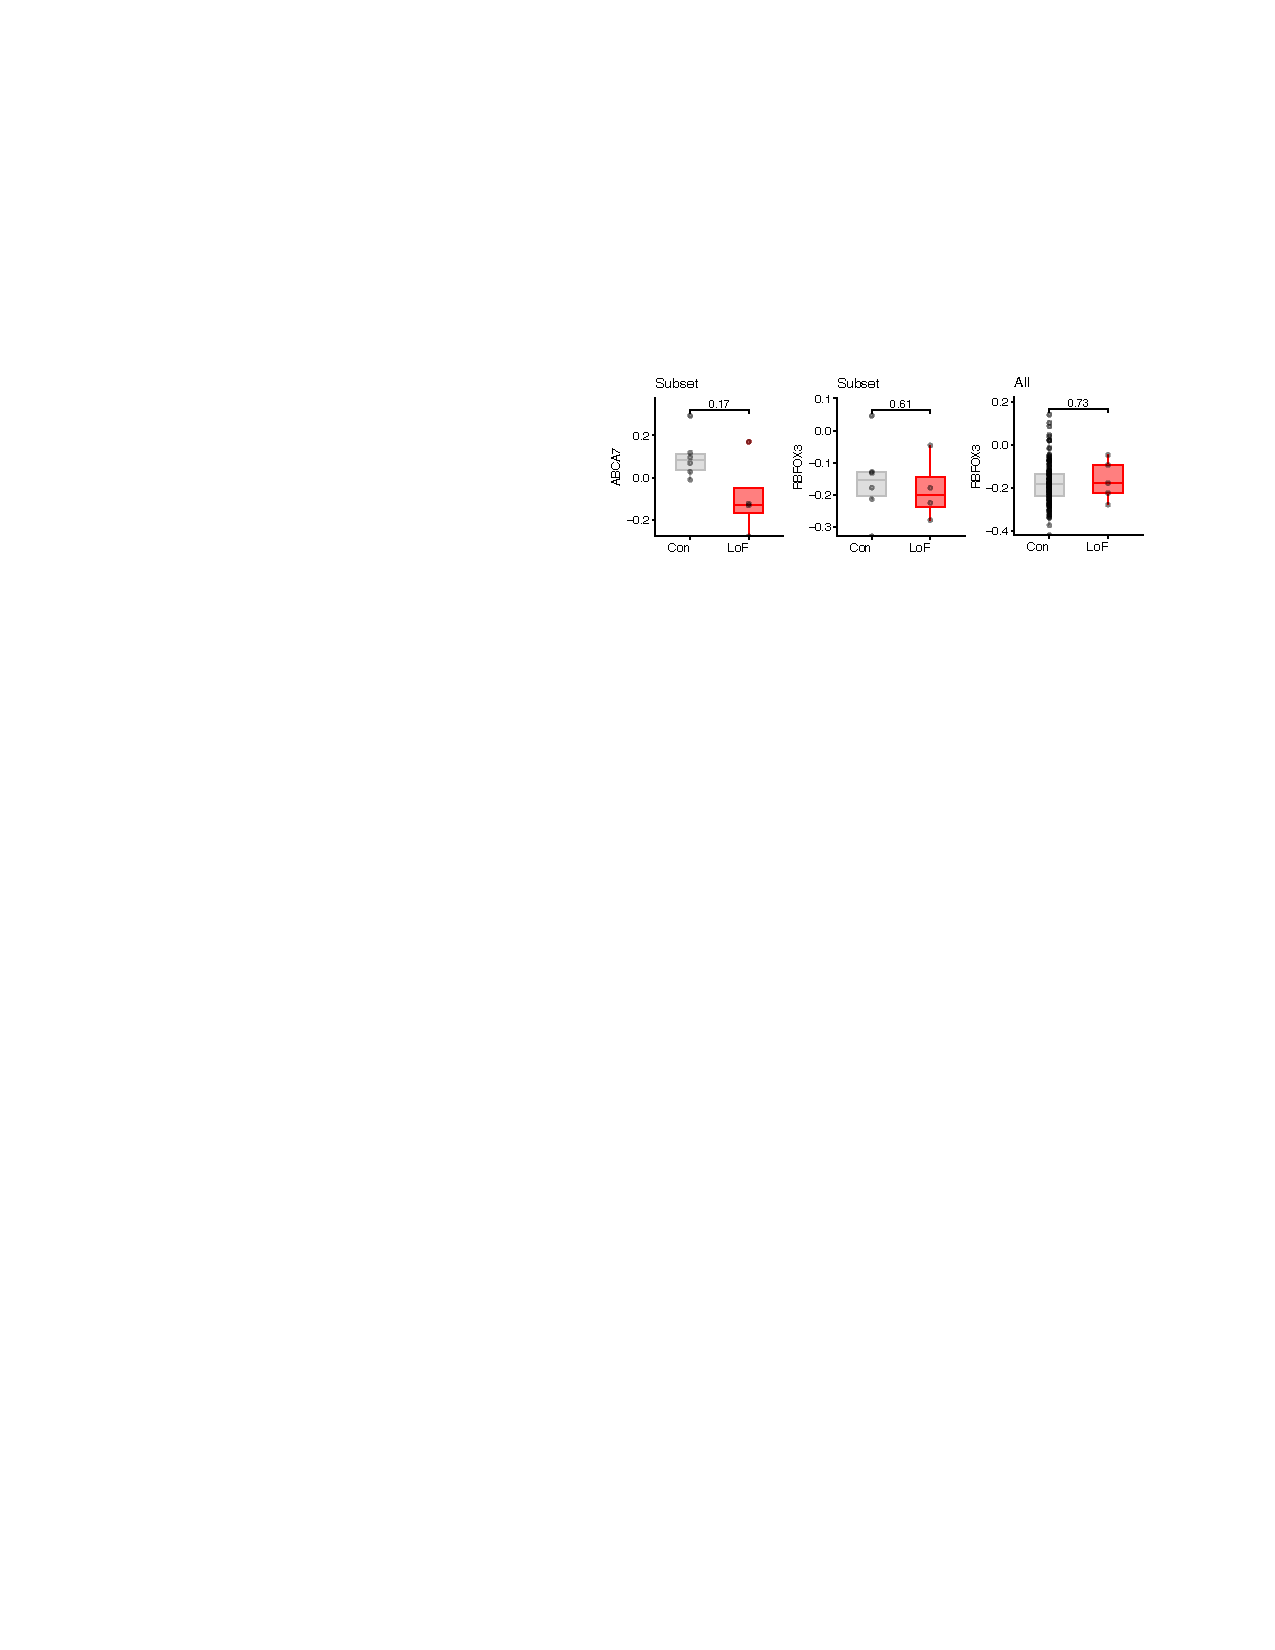
\includegraphics[width=\textwidth]{./extended_plots/protein_levels_extended.pdf}        
        \end{subfigure}  
    \end{subfigure}  
    \begin{subfigure}[t]{\textwidth}
        \caption{}
        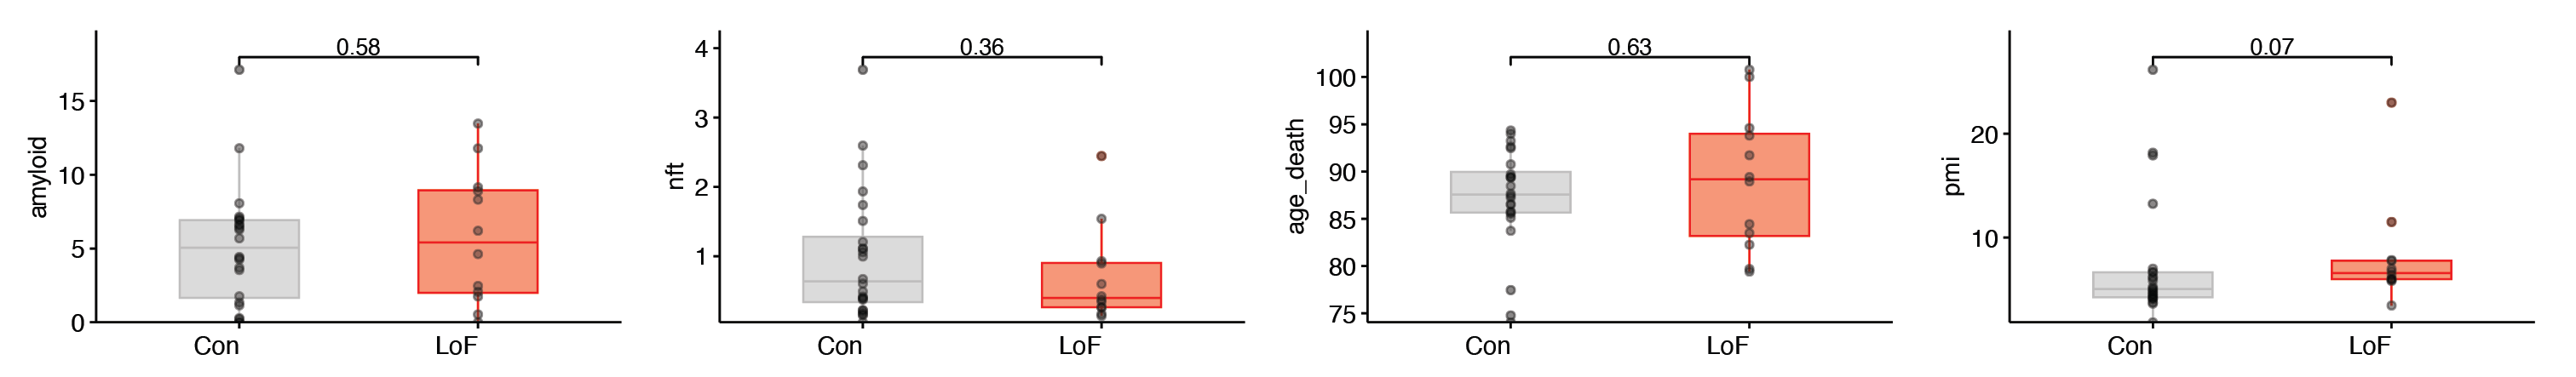
\includegraphics[width=\textwidth]{./extended_plots/batch_cont_var.png}        
    \end{subfigure}  
    \begin{subfigure}[t]{\textwidth}
        \caption{}
        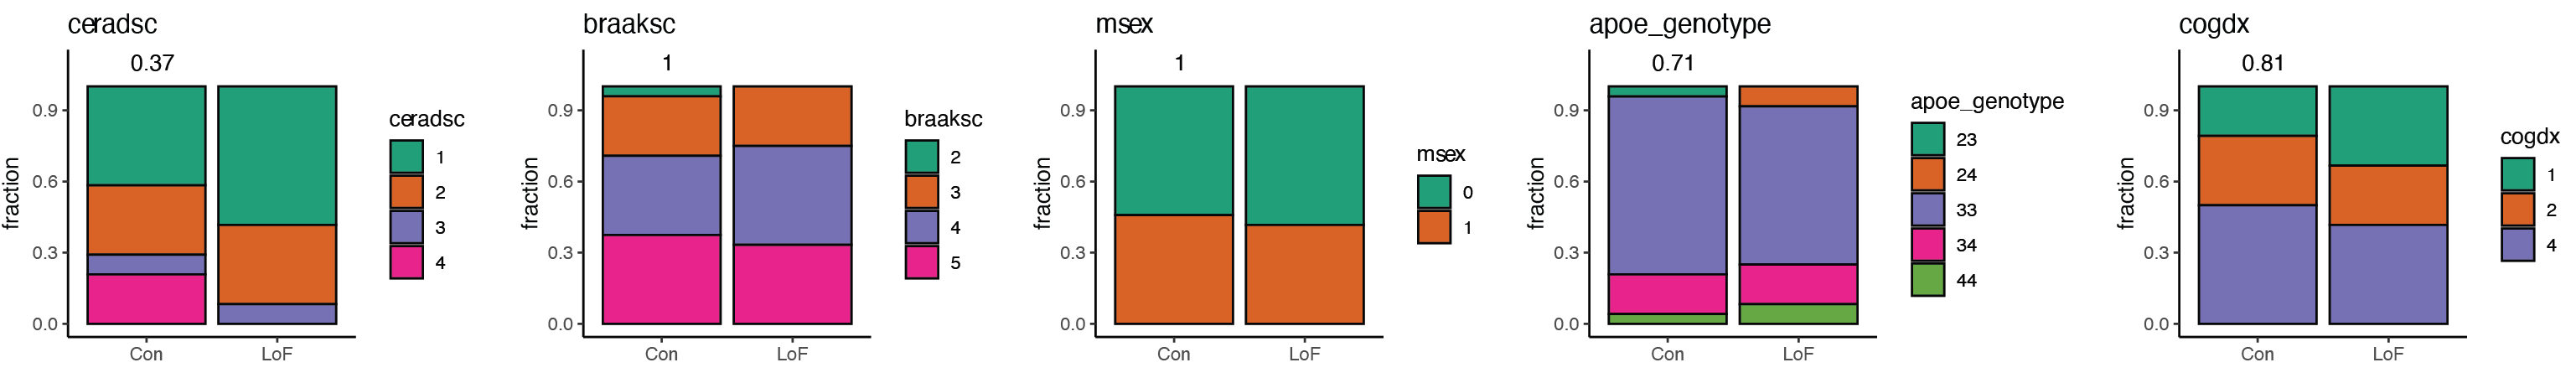
\includegraphics[width=\textwidth]{./extended_plots/batch_categorical_vars.png}        
    \end{subfigure}  
    \caption{
        \textbf{Overview of Human snRNA-Sequencing Cohort.}\\[1ex]
        (A) Sanger sequencing of ABCA7 LoF variants in prefrontal cortex genomic DNA samples from 3 ABCA7 LoF carriers and 3 controls from the snRNA-seq cohort. Sequencing confirmed heterozygosity of the indicated variant in LoF samples, with variant location marked by a black box. 
        (B) Example plots validating matches between whole genome sequencing (WGS) and snRNA-seq libraries. Each plot shows the concordance of homo- and heterozygous SNP calls between WGS and snRNA-seq data for a single individual. Matches between WGS SNP calls and snRNA-seq BAM inferred SNP calls are indicated by extreme outliers. Expected (i.e., correct) matches are indicated in blue/purple. 
        (C) Protein levels from post-mortem human prefrontal cortex (see Table~\ref{tab:external_datasets} for external dataset used) showing ABCA7 protein levels (left) and NeuN (RBFOX3) levels (middle) for a subset of individuals in the snRNA-seq cohort (N=6 control and N=4 ABCA7 LoF carriers). The right panel shows NeuN (RBFOX3) protein levels by genotype in all available control samples (N=180) vs. ABCA7 LoF carriers (N=5). 
        (D) Distributions of continuous metadata variables (see Supplementary Text for descriptions) for control individuals (N=24) vs. ABCA7 LoF carriers (N=12). For panels C and D, boxes indicate dataset quartiles per condition, and whiskers extend to the most extreme data points not considered outliers (i.e., within 1.5 times the interquartile range from the first or third quartile). 
        (E) Distributions of discrete metadata variables for control individuals (N=24) vs. ABCA7 LoF carriers (N=12). Con=control, LoF=ABCA7 loss-of-function. P-values in panels C and D were computed by two-sided Wilcoxon rank sum test. P-values in panel E were computed by two-sided Fisher’s exact test.
    }
    \label{fig:snRNA_cohort}
\end{figure}
\clearpage

\begin{figure}[H]
    \begin{subfigure}[t]{\textwidth}
        \caption{}
        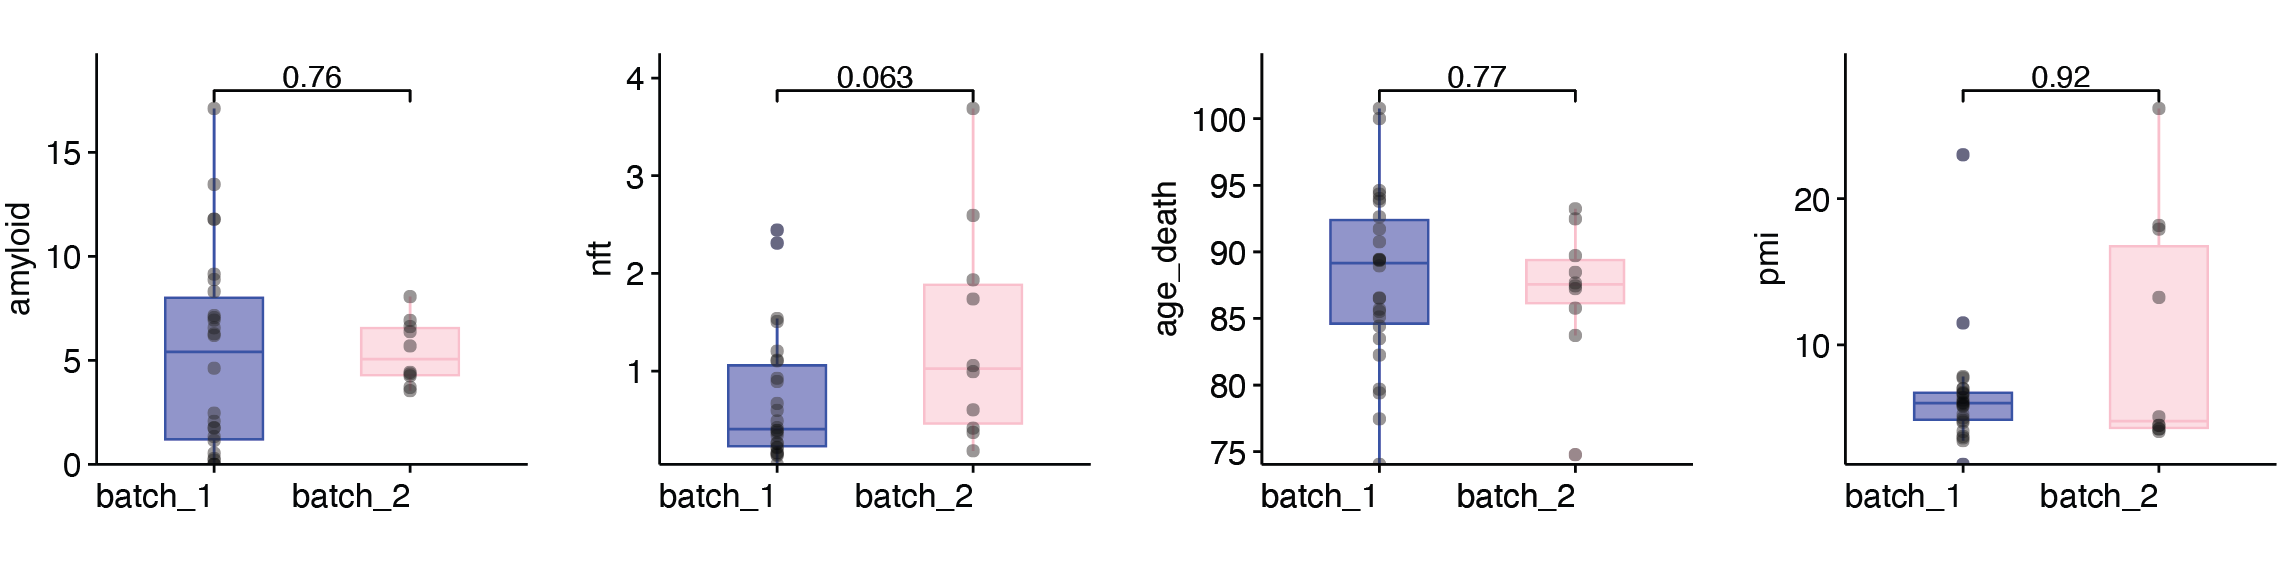
\includegraphics[width=\textwidth]{./extended_plots/seq_batch_cont.png}        
    \end{subfigure}
    \begin{subfigure}[t]{\textwidth}
        \caption{}
        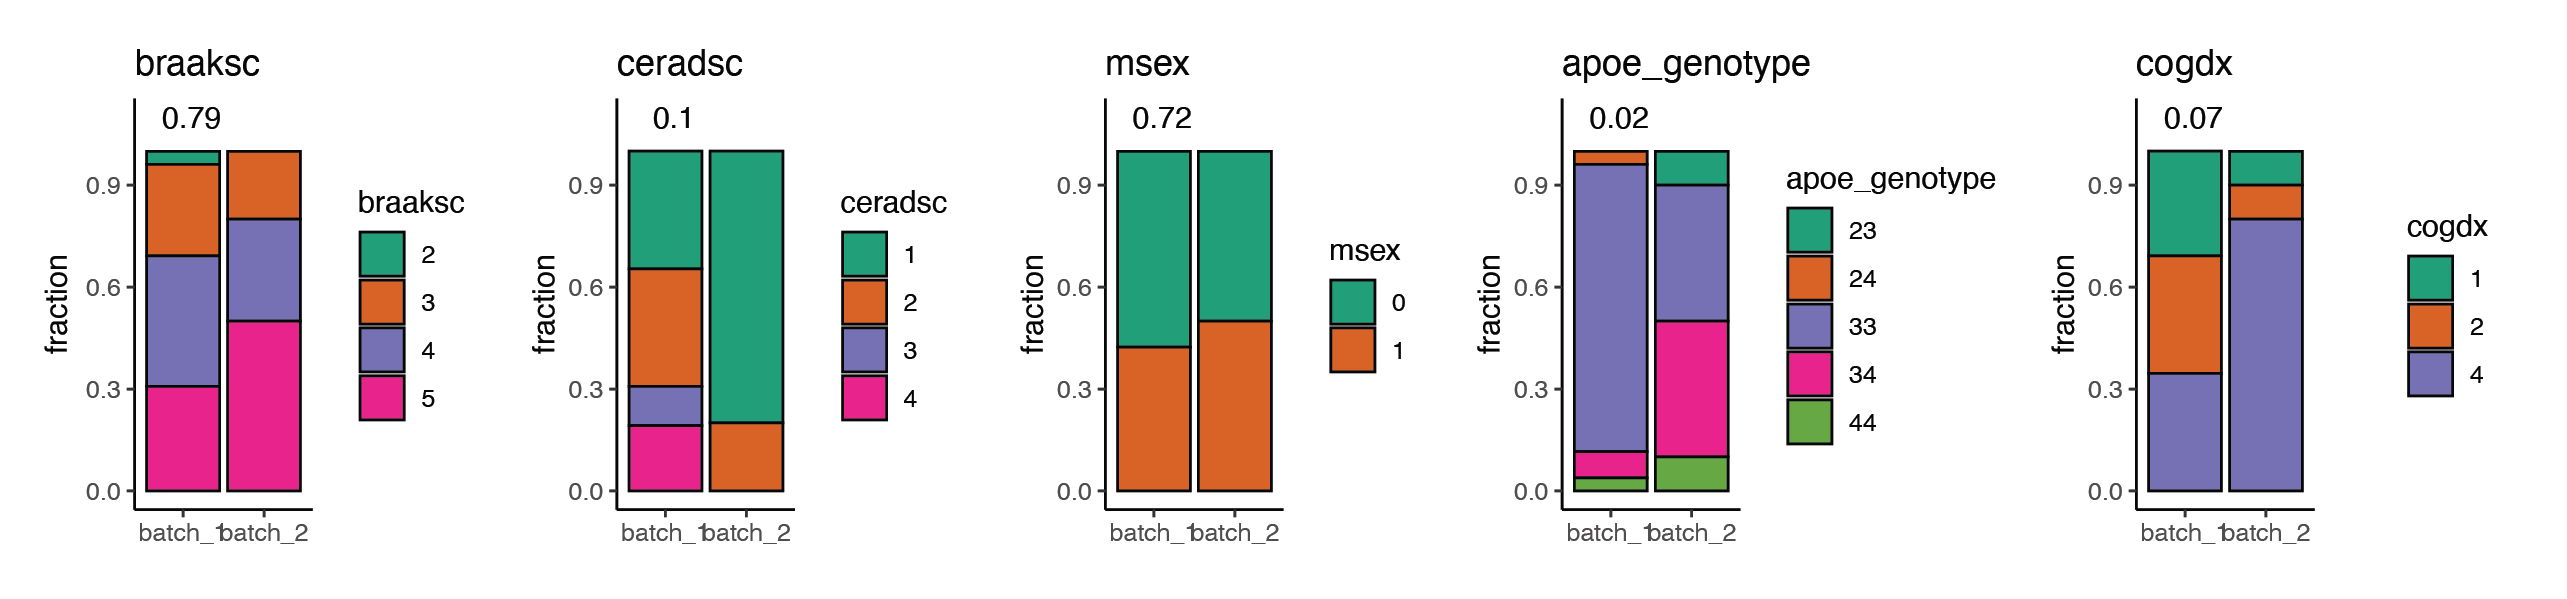
\includegraphics[width=\textwidth]{./extended_plots/seq_batch_cat.png}        
    \end{subfigure}  
    \begin{subfigure}[t]{\textwidth}
        \caption{}
        \includegraphics[width=\textwidth]{./extended_plots/additional_projections.png}        
    \end{subfigure}   
    \caption{
        \textbf{Overview of snRNA-sequencing Batch Correction and Data Quality.}\\
    }
    \label{fig:snRNA_quality_annotation}
\end{figure}
\begin{itemize}
    \item[\textbf{(A,B)}] Distributions of continuous (A) and discrete (B) metadata variables by sequencing batch. 
    \item[\textbf{(C)}] Two-dimensional UMAP projection of snRNA-seq single cells from gene expression space, colored by selected variables after all rounds of quality control. 
\end{itemize}
\clearpage

\begin{figure}[H]
    \begin{subfigure}[t]{.5\textwidth}
        \begin{subfigure}[t]{.45\textwidth}
            \caption{}
            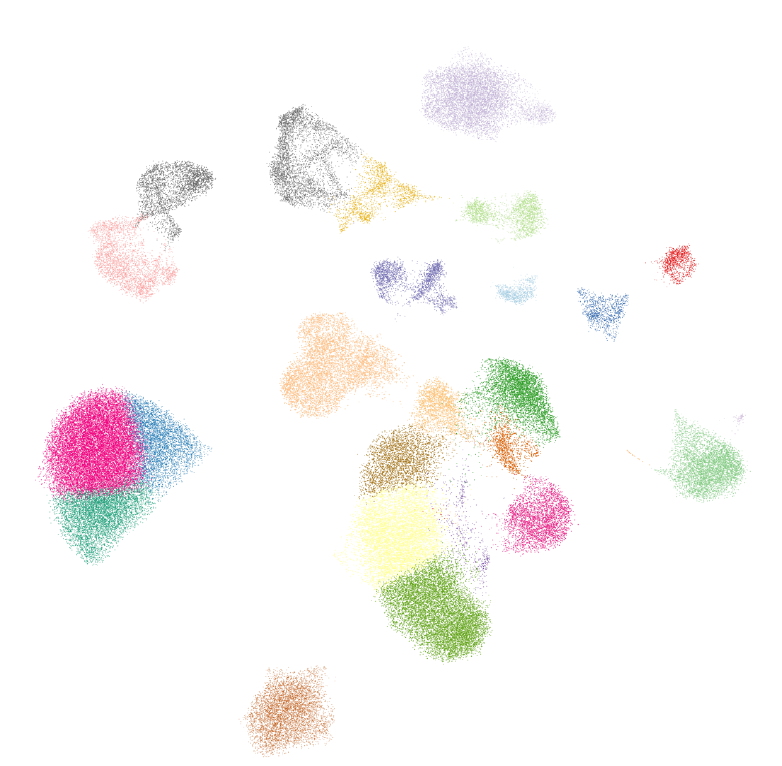
\includegraphics[width=\textwidth]{./extended_plots/cell_proj_with_leiden.png}        
        \end{subfigure}
        \hspace{0.5cm}  
        \begin{subfigure}[t]{.45\textwidth}
            \caption{}
            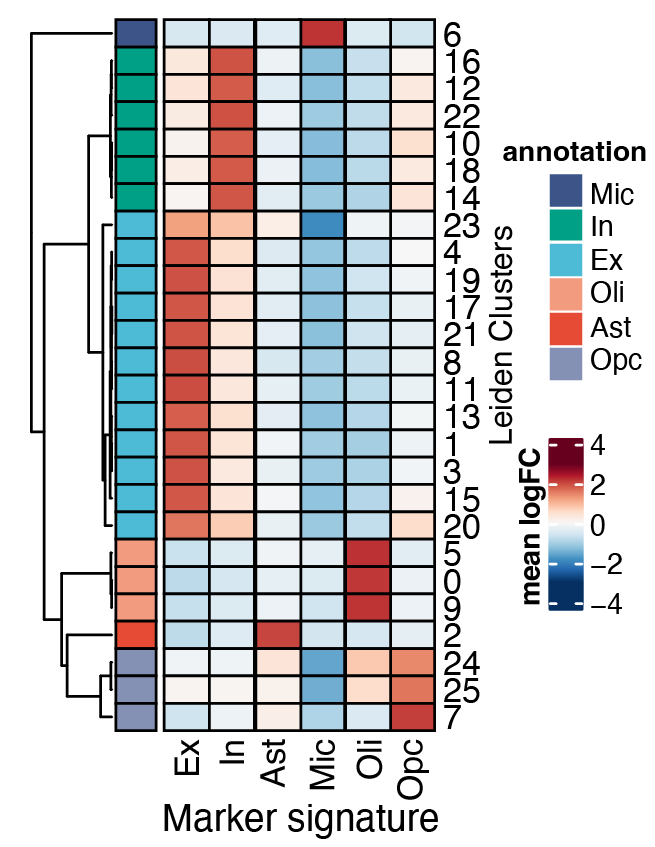
\includegraphics[width=\textwidth]{./extended_plots/leiden_heatmap.png}        
        \end{subfigure}   
        \begin{subfigure}[t]{.3\textwidth}
            \caption{}
            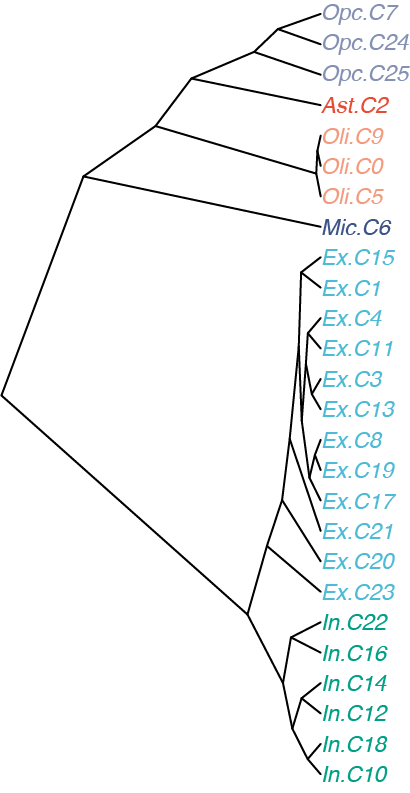
\includegraphics[width=\textwidth]{./extended_plots/hierarchical_tree.png}        
        \end{subfigure}  
        \hspace{1cm}
        \begin{subfigure}[t]{.45\textwidth}
            \caption{}
            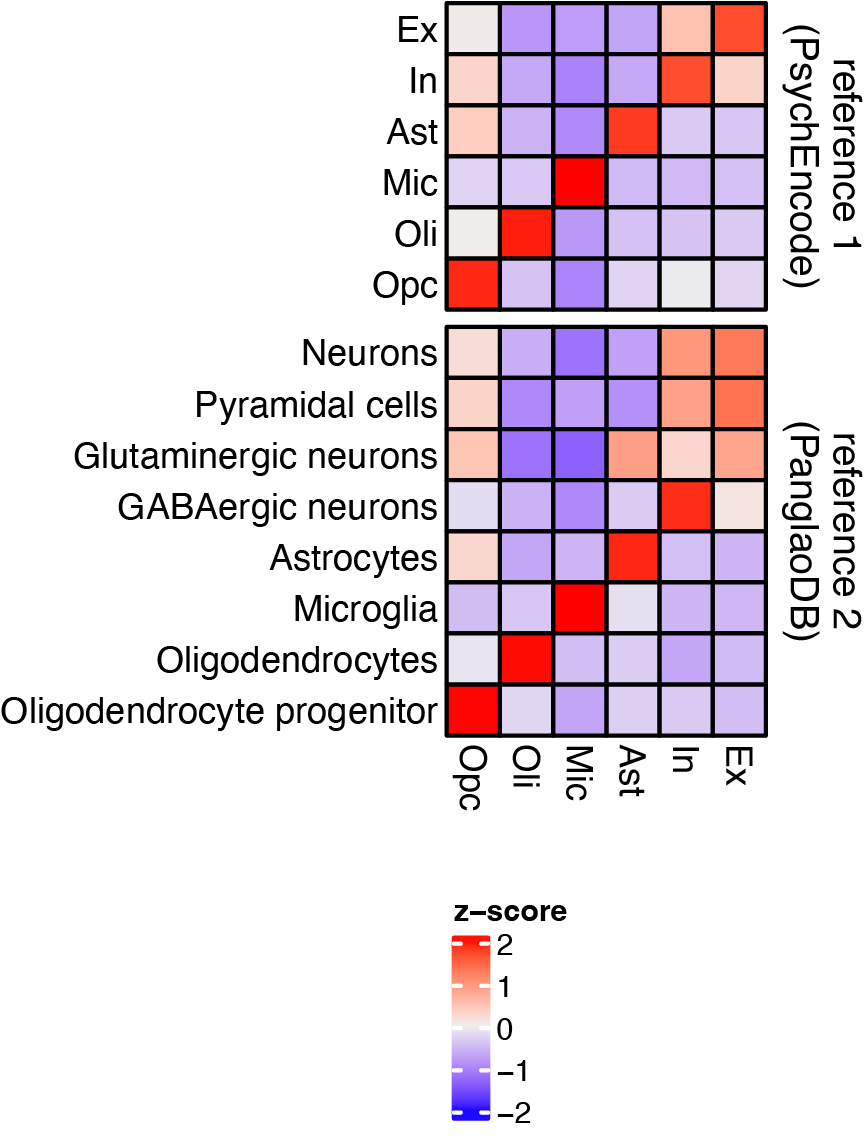
\includegraphics[width=\textwidth]{./extended_plots/marker_hmap.png}        
        \end{subfigure}  
    \end{subfigure}
    \hspace{2cm}  
    \begin{subfigure}[t]{.25\textwidth}
        \caption{}
        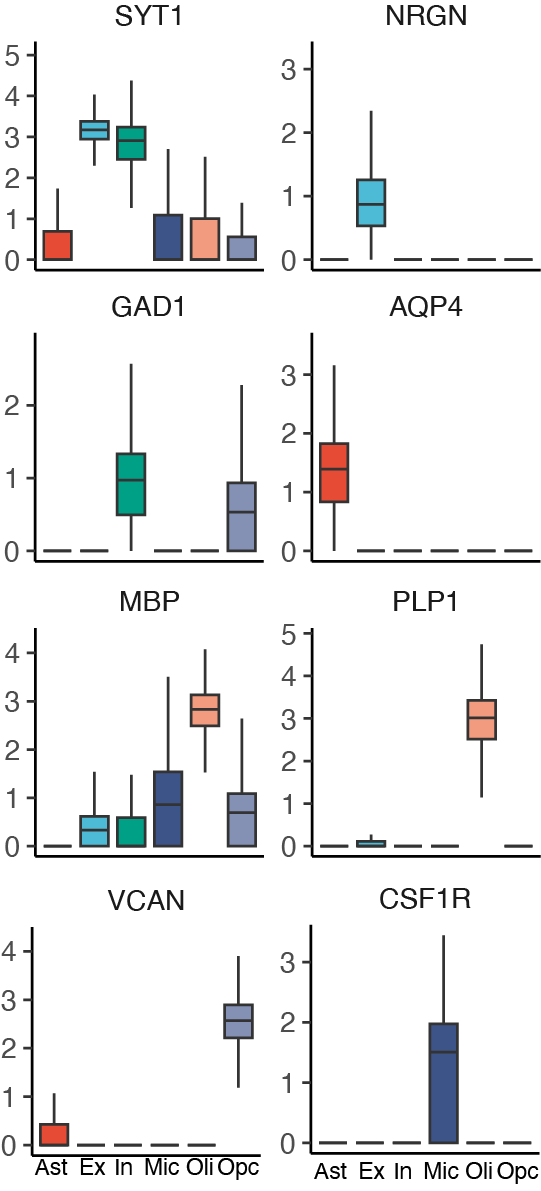
\includegraphics[width=\textwidth]{./extended_plots/marker_boxplot.png}        
    \end{subfigure}    
    \par
    \begin{subfigure}[t]{.15\textwidth}
        \caption{}
        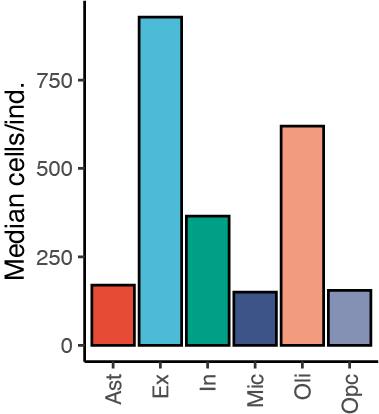
\includegraphics[width=\textwidth]{./extended_plots/median_cells.png}        
    \end{subfigure} 
    \hspace{0.5cm}   
    \begin{subfigure}[t]{.25\textwidth}
        \caption{}
        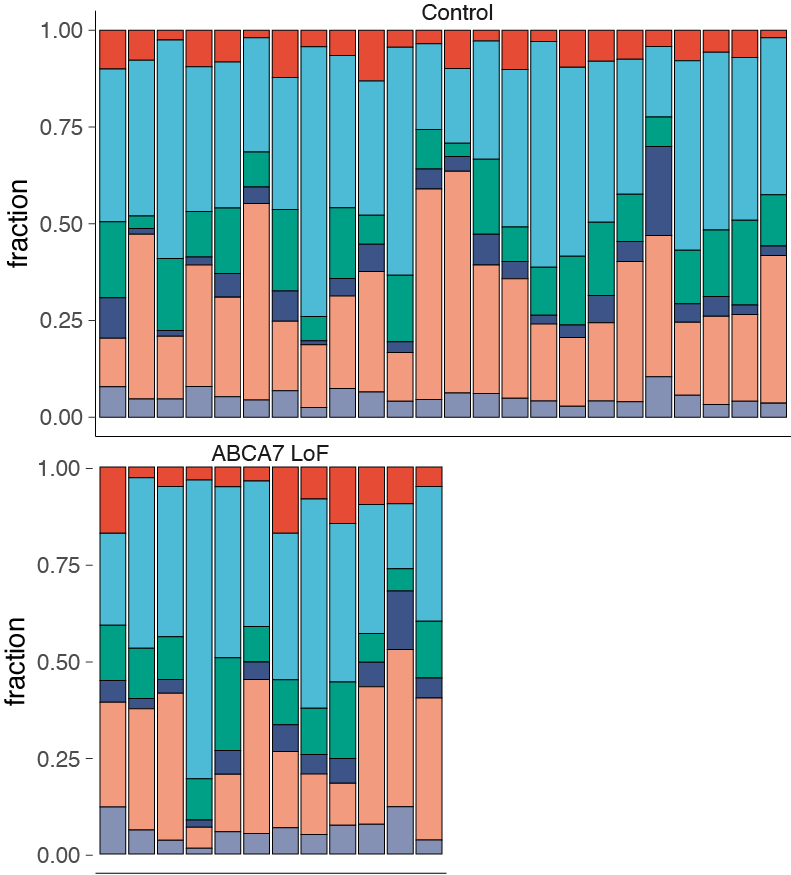
\includegraphics[width=\textwidth]{./extended_plots/individual_fractions.png}        
    \end{subfigure}  
    \hspace{0.5cm}   
    \begin{subfigure}[t]{.25\textwidth}
        \caption{}
        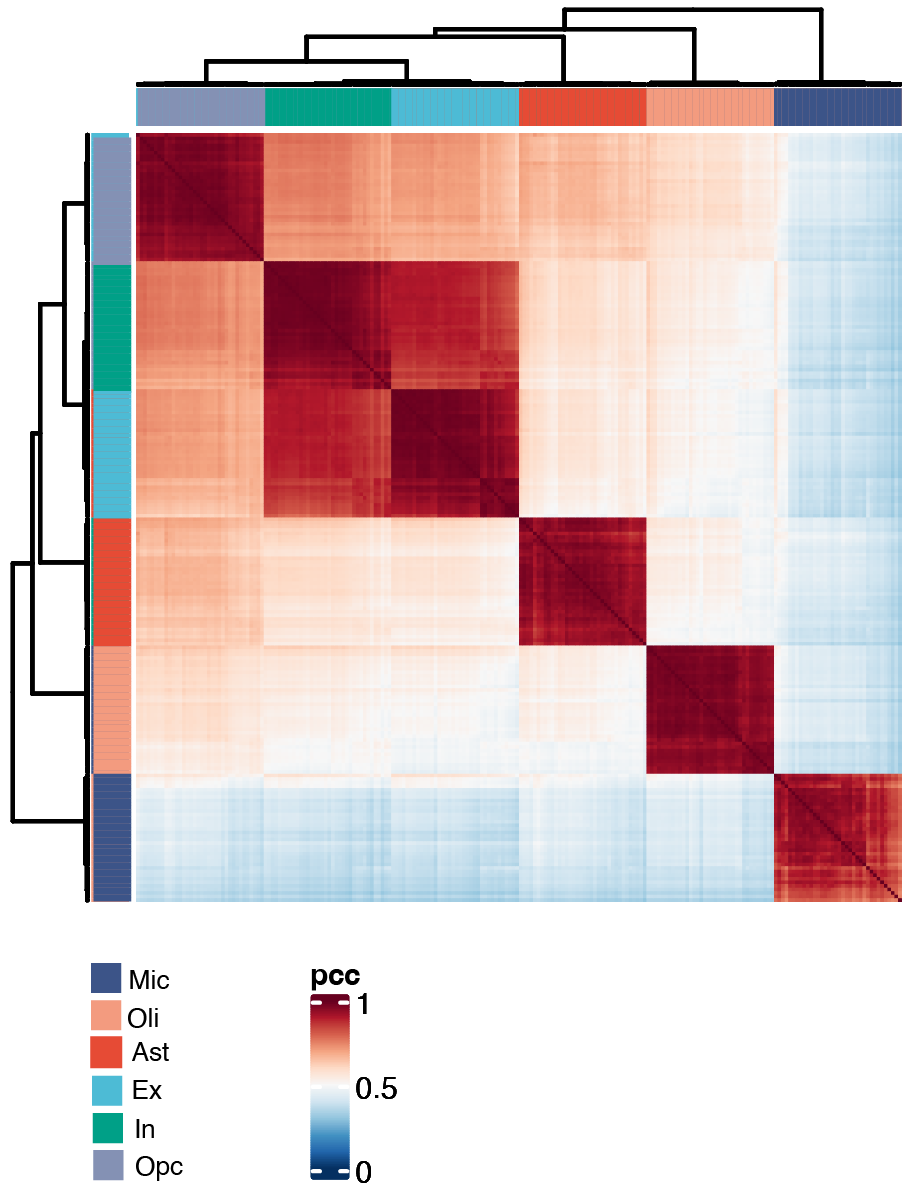
\includegraphics[width=\textwidth]{./extended_plots/celltype_heatmap.png}        
    \end{subfigure}  
    \hspace{0.5cm}
    \begin{subfigure}[t]{.15\textwidth}
        \caption{}
        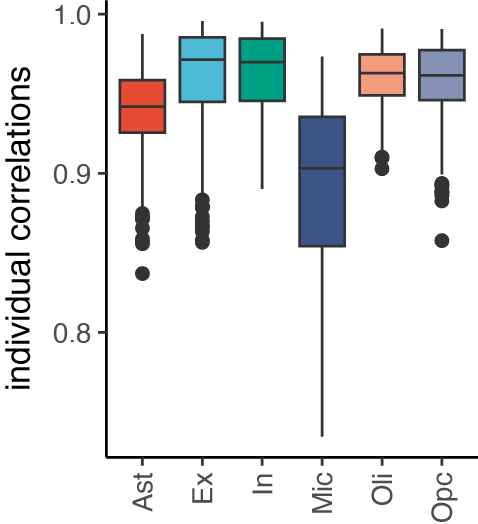
\includegraphics[width=\textwidth]{./extended_plots/individual_correlations.png}        
    \end{subfigure}       
    \caption{
        \textbf{Overview of snRNA-sequencing Cell Type Annotations.}\\
    }
    \label{fig:snRNA_quality_annotation}
\end{figure}
\begin{itemize}
    \item[\textbf{(A)}] Two-dimensional UMAP projections of individual cells from gene expression space, colored by Leiden clusters. 
    \item[\textbf{(B)}] Average marker gene expression (per-cluster mean log(fold-change)) for all marker genes for the cell type indicated along the x-axis. Log(fold-changes) are computed for the cluster of interest vs. all remaining clusters. Reference 1 (Table 2) marker genes were used. 
    \item[\textbf{(C)}] Cladogram visualizing subcluster relationships based on pairwise distances between per-cluster gene expression profiles. 
    \item[\textbf{(D)}] Average marker gene expression profiles (x-axis) per major cell type annotation (y-axis) for two marker gene references. 
    \item[\textbf{(E)}] Per-cell distribution of select marker gene expression by cell type. Y-axis indicates log counts. 
    \item[\textbf{(F)}] Median number of cells per cell type per individual. 
    \item[\textbf{(G)}] Cell type fraction by individual. 
    \item[\textbf{(H)}] Heatmap of individual-level gene expression correlations by cell type. 
    \item[\textbf{(I)}] Boxplot of individual-level gene expression correlations by cell type. 
\end{itemize}
For all panels, p-values for all continuous variables were computed by two-sided Wilcoxon rank sum test. 
P-values for all discrete variables were computed by two-sided Fisher’s exact test. 
For A, I, M boxes indicate per-condition dataset quartiles, and whiskers extend to the most extreme data points not considered outliers (i.e., within 1.5 times the interquartile range from the first or third quartile).
\clearpage

\begin{figure}[H]
    \begin{subfigure}[t]{1\textwidth}
        \caption{}
        \centering
        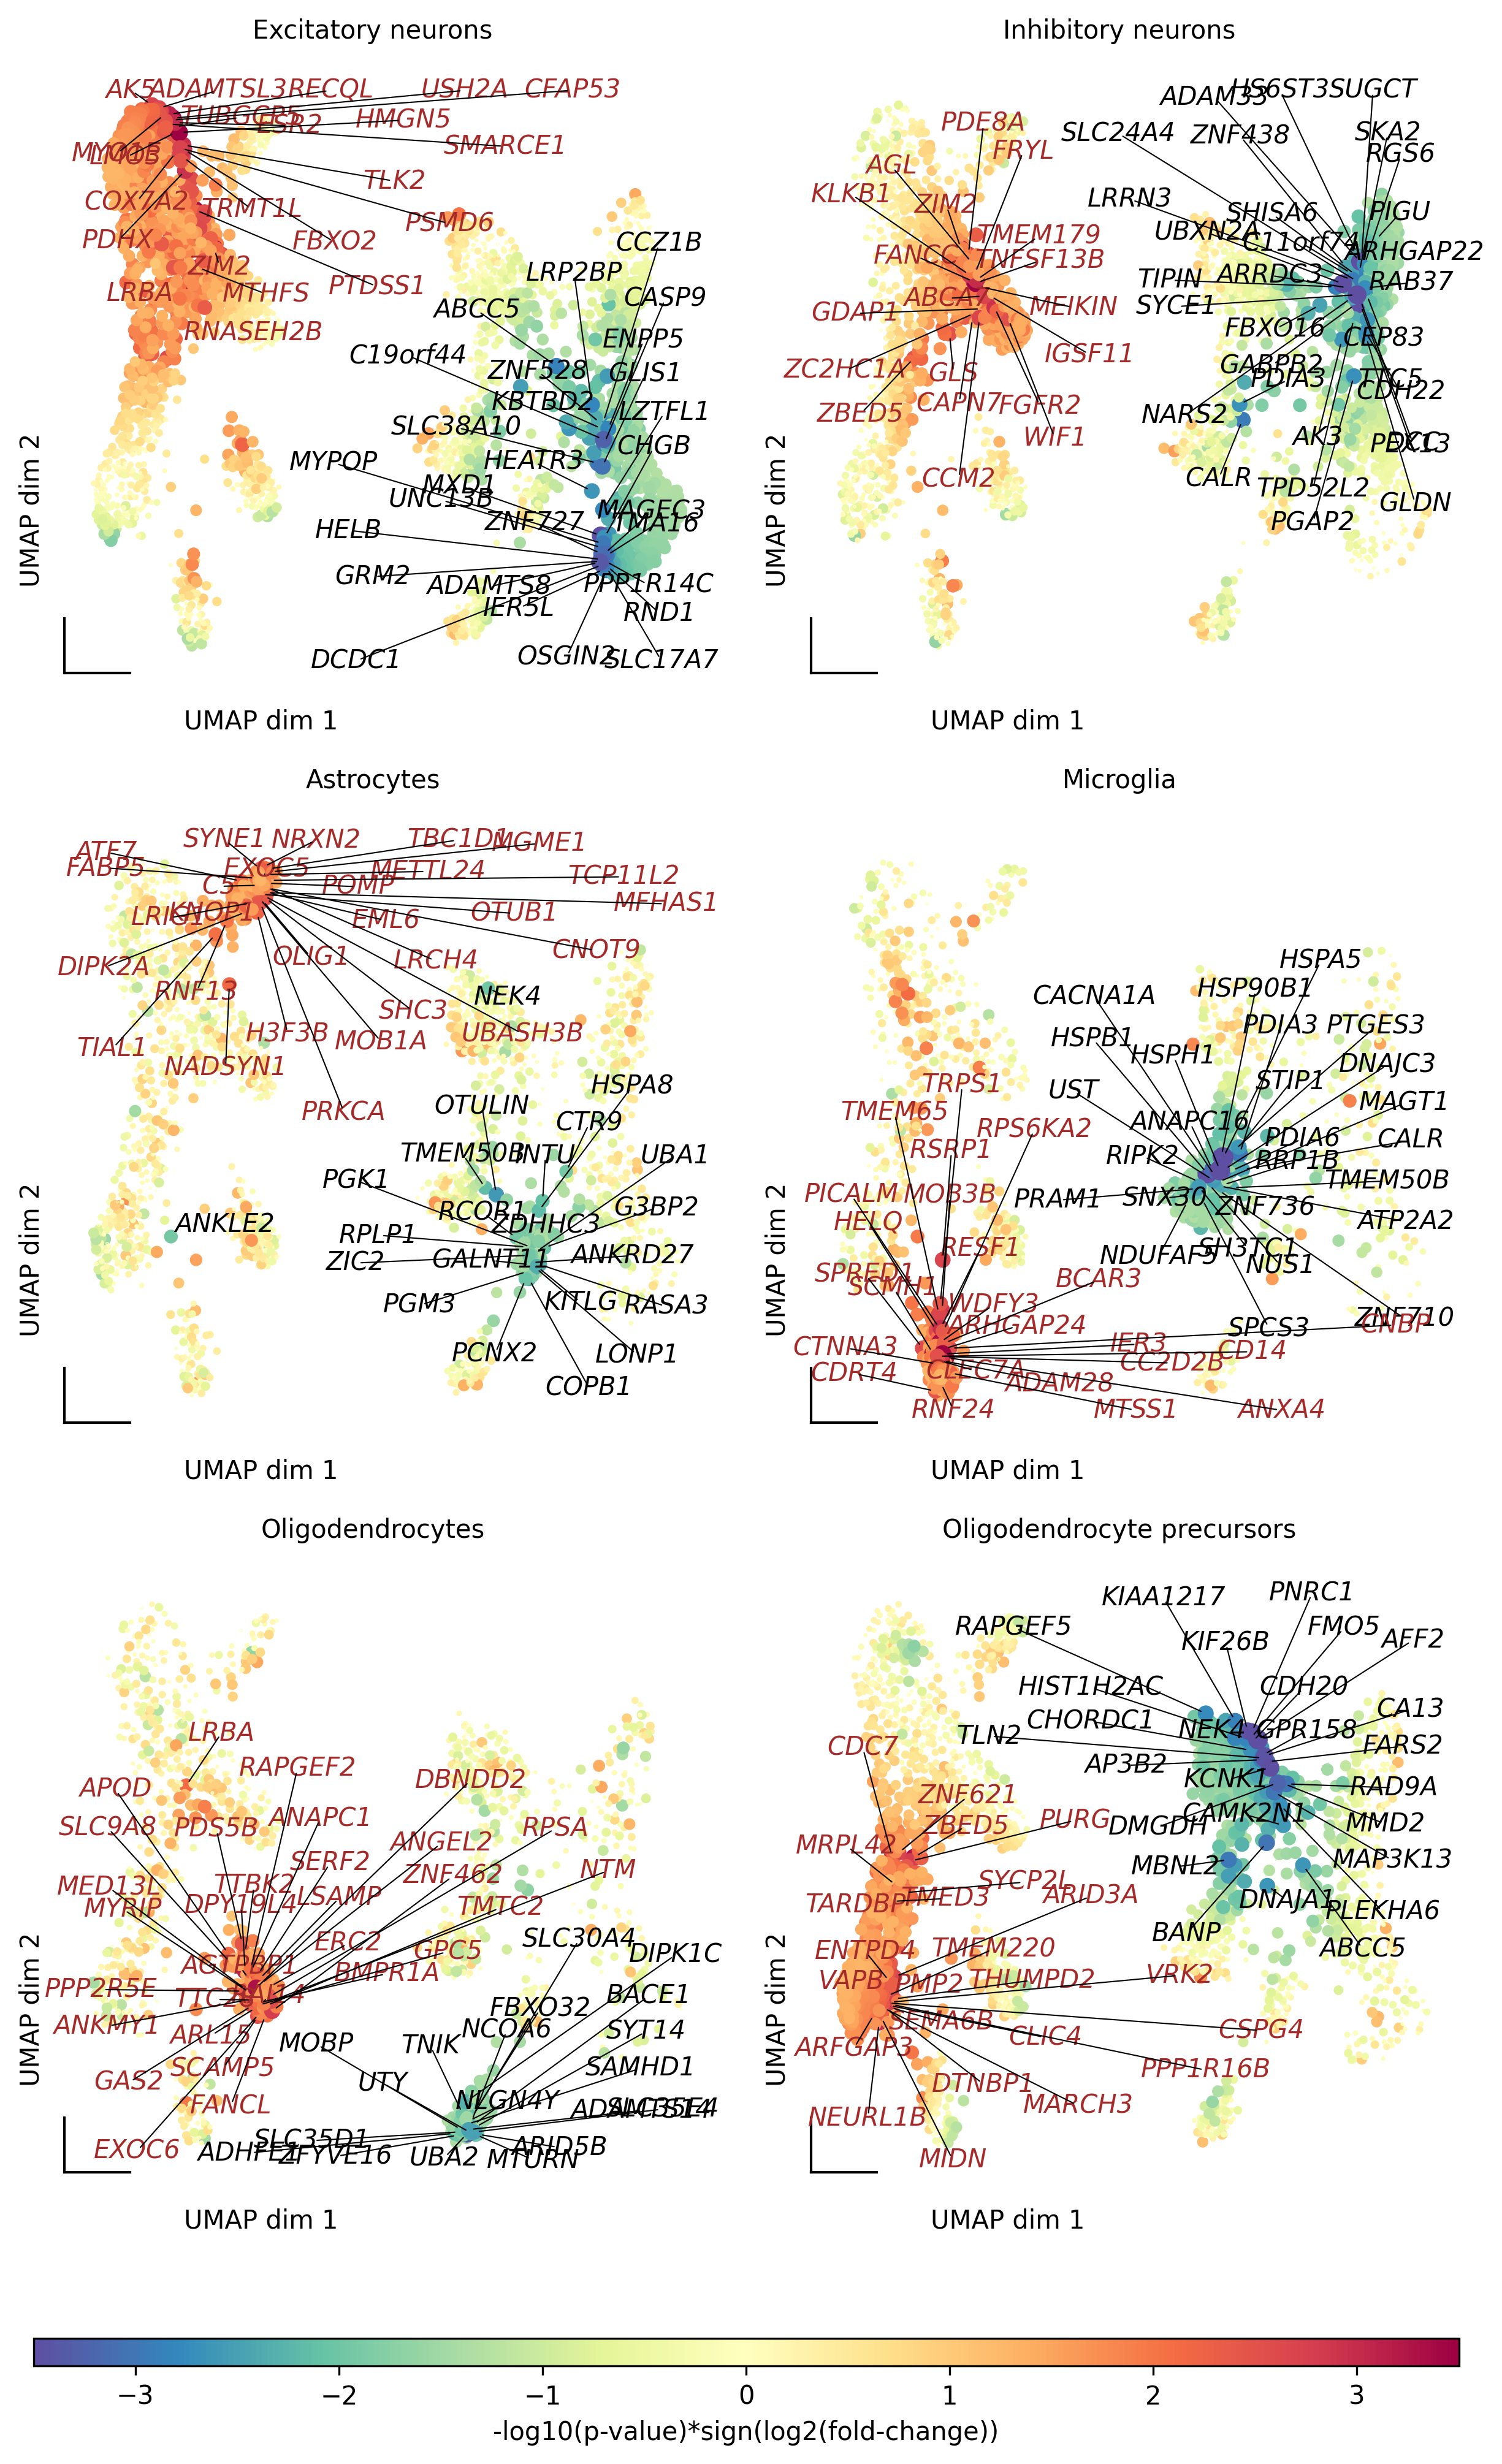
\includegraphics[width=0.7\textwidth]{./extended_plots/umap_projection_more_genes.png}        
    \end{subfigure}    
    \caption{
        \textbf{Annotated projections of gene scores.}\\
    }
    \label{fig:snRNAseq_gene_scores}
\end{figure}

\begin{itemize}
    \item[\textbf{(A)}] Enlarged view of the UMAP projection of Figure~\ref{fig:main_atlas}E, showing the top 20 genes by absolute score ($|S|$) for each cell type. 
\end{itemize}

\clearpage
\begin{figure}[ht]
    \begin{subfigure}[t]{.3\textwidth}
        \caption{}
        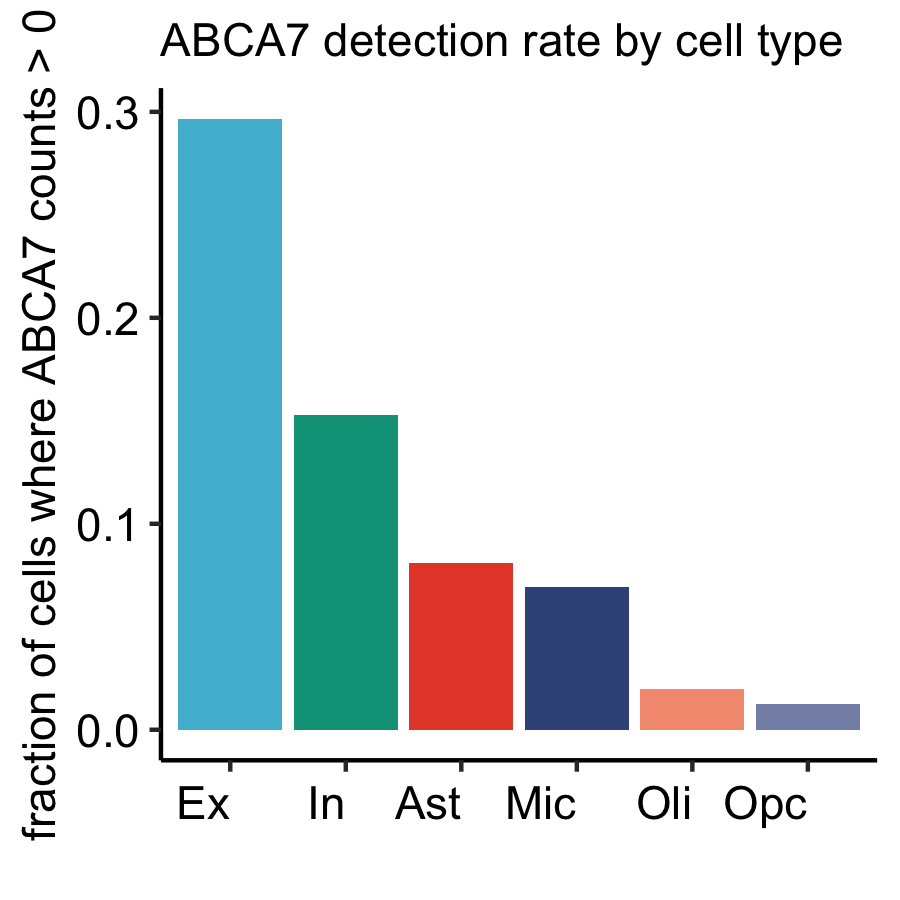
\includegraphics[width=\textwidth]{./extended_plots/abca7_detection_rate.png}        
    \end{subfigure}
    \par
    \begin{subfigure}[t]{1\textwidth}
        \caption{}
        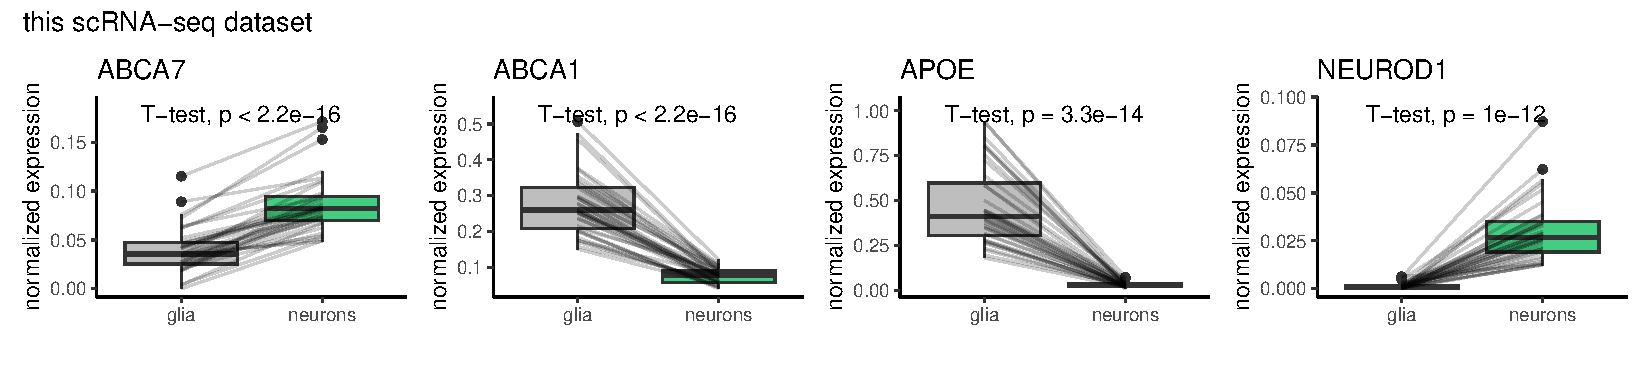
\includegraphics[width=\textwidth]{./extended_plots/scRNAseq_bulk_rna.pdf}        
    \end{subfigure}
    \begin{subfigure}[t]{1\textwidth}
        \caption{}
        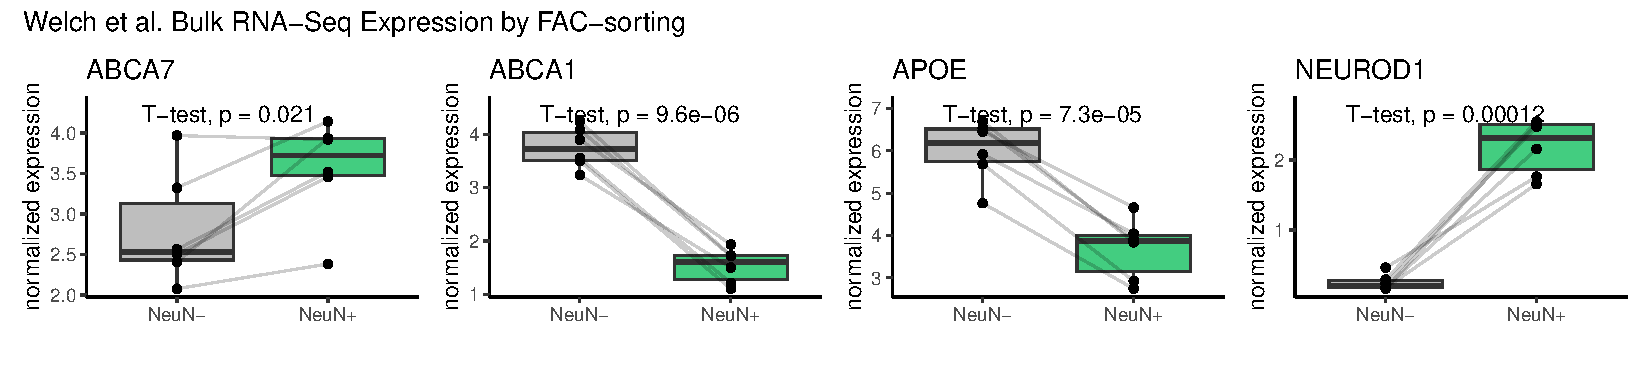
\includegraphics[width=\textwidth]{./extended_plots/welch_et_al_bulk_rna.pdf}        
    \end{subfigure}
    \caption{
        \textbf{Neuronal Expression of ABCA7 in the Post-mortem Human Brain.}\\[1ex]
        (A) Per cell type ABCA7 detection rate of major cell types in the post-mortem PFC as quantified by snRNA-seq. 
        (B) Normalized expression of indicated gene in glial cells (per-individual mean expression profiles across Oli, Opc, Ast, Mic) vs. neuronal cells (per-individual mean expression profiles across Ex and In) from post-mortem snRNA-seq data. 
        (C) Normalized expression of indicated genes in NeuN- vs. NeuN+ cells (N=6 individuals, from \cite{Welch2022-aa}; see Table 2). All p-values are computed by paired two-sided t-test. Boxes indicate per-condition dataset quartiles, and whiskers extend to the most extreme data points not considered outliers (i.e., within 1.5 times the interquartile range from the first or third quartile).
    }
    \label{fig:abca7_expression}
\end{figure}

\clearpage
\begin{figure}[ht]
    \begin{subfigure}[t]{0.5\textwidth}
        \caption{}
        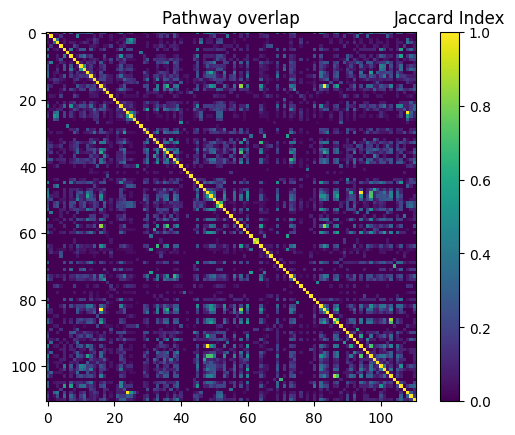
\includegraphics[width=\textwidth]{./extended_plots/jaccard_mat_sub.png}        
    \end{subfigure}
    \begin{subfigure}[t]{0.5\textwidth}
        \caption{}
        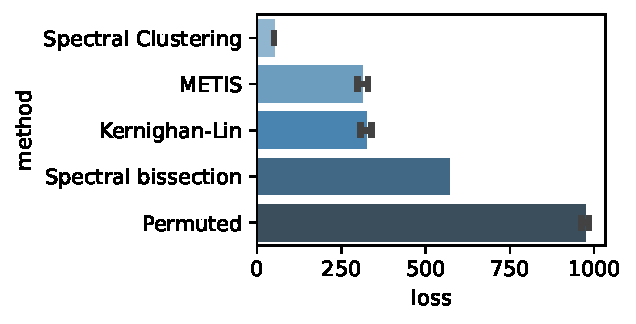
\includegraphics[width=\textwidth]{./extended_plots/partitioning_losses.pdf}        
    \end{subfigure}
    \begin{subfigure}[t]{1\textwidth}
        \caption{}
        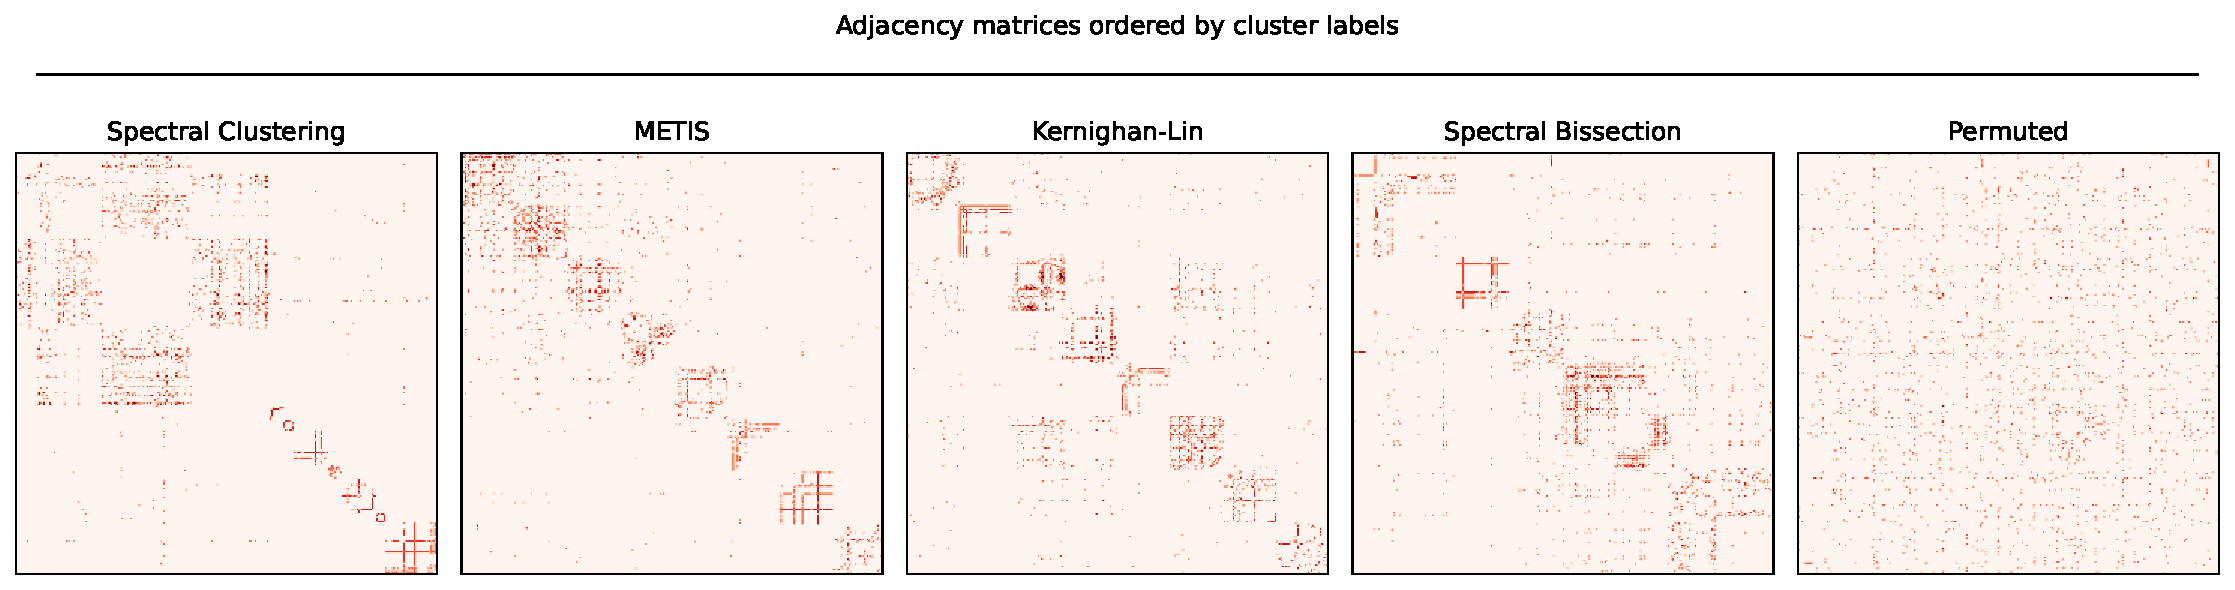
\includegraphics[width=\textwidth]{./extended_plots/adjacency_matrices_ordered_by_cluster_labels.pdf}        
    \end{subfigure}
    \begin{subfigure}[t]{0.33\textwidth}
        \caption{}
        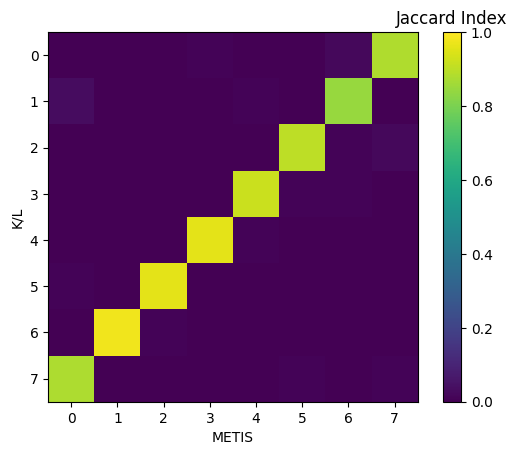
\includegraphics[width=\textwidth]{./extended_plots/argmins_jaccard.png}        
    \end{subfigure}
    \begin{subfigure}[t]{0.33\textwidth}
        \caption{}
        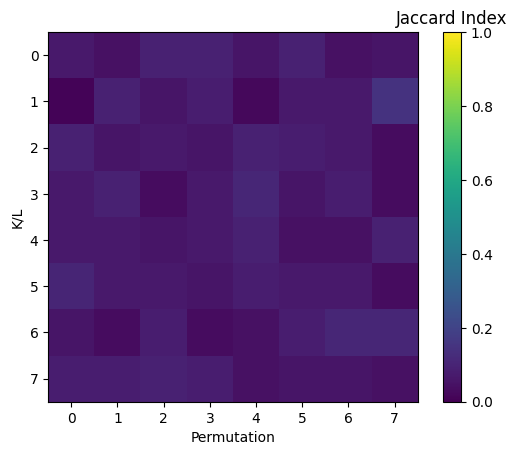
\includegraphics[width=\textwidth]{./extended_plots/random_jaccard.png}        
    \end{subfigure}
    \begin{subfigure}[t]{0.33\textwidth}
        \caption{}
        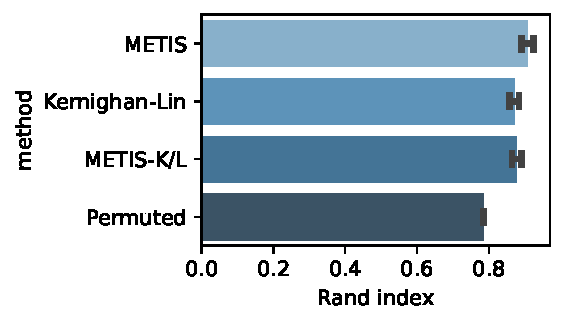
\includegraphics[width=\textwidth]{./extended_plots/rand_indices.pdf}        
    \end{subfigure}
    \caption{
        \textbf{Benchmarking Partitioning and Clustering Algorithms for Gene-Pathway Grouping.}\\[1ex]
        (A) Jaccard indices quantifying overlap of genes for all 111 pathways in Figure~\ref{fig:main_excitatory}B (see Methods; Supplementary Text). 
        (B) Average loss (total cut size; see Methods) associated with applying each algorithm (spectral clustering (SC), METIS, Kernighan-Lin (K/L), spectral bisection (SB), or random permutation) to G (with 379 vertices; see Methods) over 1000 initiations (SC, random permutation) or $5 \times 10^5$ initiations (METIS, K/L). The SB implementation is deterministic and was run only once. Error bars indicate the standard deviation. 
        (C) Unweighted adjacency matrix for G sorted by labels assigned by the indicated algorithm. Red indicates the presence of an edge between two vertices. For each algorithm, labels corresponding to the best initiation (lowest loss) over 1000 initiations (SC, random permutation) or $5 \times 10^5$ initiations (METIS, K/L) are shown. 
        (D) Pairwise labeling consistency for the best K/L initiation and the best METIS initiation. Cluster labels corresponding to each are shown on the X- and Y-axes, respectively. Each color entry indicates the fraction of shared vertices per cluster across two initiations. Consistency is quantified using the Jaccard Index (JI). $\text{JI} = \frac{|A \cap B|}{|A \cup B|}$, where A and B are two sets (i.e., cluster A from initiation \#1 and cluster B from initiation \#2). 
        (E) Same as (D), but comparing the best K/L initiation against the best random permutation initiation. 
        (F) Average Rand index (RI) for all pairwise initiations from (B). “METIS,” “Kernighan-Lin,” and “Permuted” labels on the Y-axis indicate the average RI (consistency across two sets of labels) for all combinations of initiations within the specified algorithm. “METIS-K/L” indicates the average RI for all combinations of initiations across the METIS and Kernighan-Lin algorithms. Error bars indicate standard deviations. ($\text{RI} = \frac{\text{number of agreeing vertex pairs}}{\text{number of vertex pairs}}$).
    }
    \label{fig:benchmarking_clustering}
\end{figure}
\clearpage
\begin{figure}[H]
    \begin{subfigure}[t]{.4\textwidth}
        \caption{}
        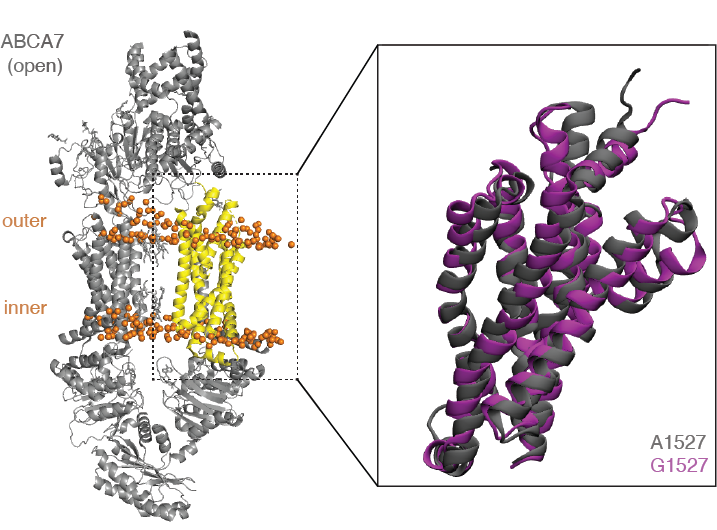
\includegraphics[width=\textwidth]{../paper/extended_plots/abca7_structure_with_inset.png}        
    \end{subfigure}
    %\hspace{1cm}
    \begin{subfigure}[t]{.25\textwidth}
        \caption{}
        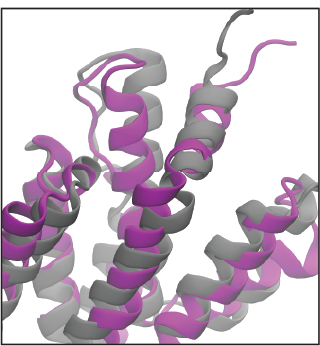
\includegraphics[width=\textwidth]{../paper/extended_plots/abca7_structure_inset_only.png}        
    \end{subfigure}
    \begin{subfigure}[t]{.33\textwidth}
        \caption{}
        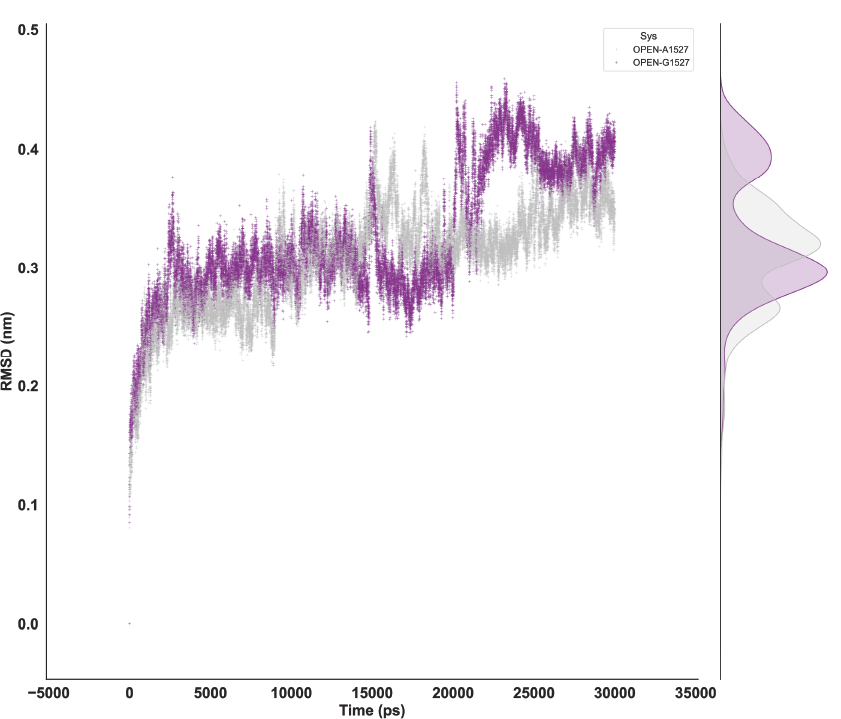
\includegraphics[width=\textwidth]{../paper/extended_plots/rmsd_time.png}        
    \end{subfigure}
    \hspace{1cm}
    \begin{subfigure}[t]{.25\textwidth}
        \caption{}
        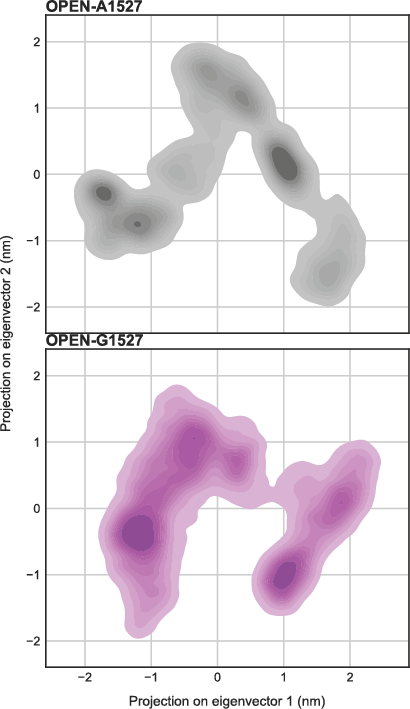
\includegraphics[width=\textwidth]{../paper/extended_plots/rmsd_projection_open.png}        
    \end{subfigure}
    \hspace{1cm}
    \begin{subfigure}[t]{.5\textwidth}
        \caption{}
        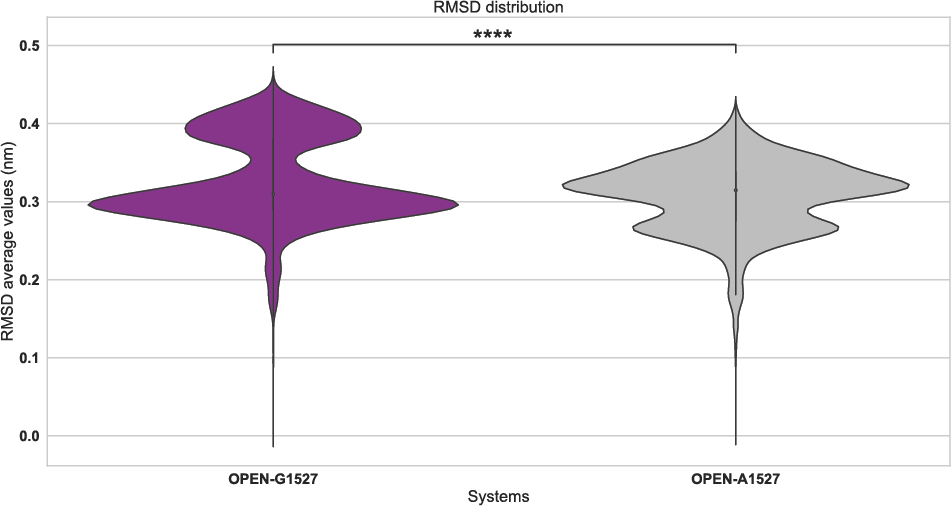
\includegraphics[width=\textwidth]{../paper/extended_plots/rmsd_volcano.png}        
    \end{subfigure}
\end{figure}
\textbf{Extended Data Fig. 6}
\clearpage


\begin{figure}[ht]
    %\centerline{\includegraphics[width=\textwidth]{./extended_plots/lipid_mitochondrial_perturbations.pdf}}
    \caption{
        \textbf{Lipid and Mitochondrial Transcriptional Perturbations in Excitatory Neurons from Human ABCA7 LoF Variant-Carriers vs. Non-Carriers.}\\[1ex]
        (A) Lipid synthesis and storage pathways perturbed in ABCA7 LoF excitatory neurons vs. control as measured by snRNA-seq on the post-mortem human PFC. Enrichments of biological processes were computed using FGSEA. Red = enrichment > 0, Blue = enrichment < 0. * = $p<0.05$. 
        (B) Schematic model showing anabolic processes feeding from the TCA cycle towards fatty acid (FA) and triglyceride (TG) synthesis. DG = diacylglyceride, PA = phosphatidic acid, PC = phosphatidylcholine, PE = phosphatidylethanolamine, PS = phosphatidylserine. * = differentially expressed in ABCA7 LoF vs. control excitatory neurons from post-mortem human brain at $p<0.05$ and $\log\text{FC}<0$. 
        (C) 𝛽-oxidation and TCA pathways perturbed in ABCA7 LoF excitatory neurons vs. control as measured by snRNA-seq on the post-mortem human PFC. Enrichments of biological processes were computed using FGSEA. Red = enrichment > 0, Blue = enrichment < 0. * = $p<0.05$. 
        (D) Schematic model showing catabolic processes feeding into the TCA cycle and oxidative phosphorylation with key genes from (C) highlighted in red or blue. * = $p<0.05$. For (A, C,) boxes indicate per-condition dataset quartiles, and whiskers extend to the most extreme data points not considered outliers (i.e., within 1.5 times the interquartile range from the first or third quartile). 
        (E, F) Transcript levels of ACLY (E) and SCP2 (F) assessed in post-mortem human PFC by RNAscope. Transcript counts per SLC17A7+ cell are reported in each bar chart. $N = 8$ individuals per genotype. Per-cell Wilcoxon rank-sum p-values are reported.
    }
    \label{fig:lipid_mitochondrial_perturbations}
\end{figure}

\begin{figure}[ht]
    \centerline{\includegraphics[width=\textwidth]{./extended_plots/differentiating_iPSC_neurons.pdf}}
    \caption{
        \textbf{Differentiating and Profiling iPSC-Derived Neurons Harboring ABCA7 PTC Variants.}\\[1ex]
        (A) Sanger sequencing chromatogram confirming single nucleotide insertion in ABCA7 exon 3 to introduce a premature termination codon into the isogenic iPSC line ABCA7 p.Glu50fs*3 using CRISPR-Cas9 gene editing. 
        (B) Sanger sequencing chromatogram confirming patient single nucleotide polymorphism in ABCA7 exon 15 to introduce a premature termination codon into the isogenic iPSC line ABCA7 p.Tyr622* using CRISPR-Cas9 gene editing. 
        (C) Normal karyotypes were observed for control, ABCA7 p.Glu50fs*3, and ABCA7 p.Tyr622* isogenic iPSC lines. 
        (D) iPSCs were plated at low density for NGN2 viral transduction. Expression of NGN2 was driven by doxycycline (DOX) induction with puromycin (PURO) selection, then re-plated to match neuronal densities. Neurons were maintained for 4 weeks (DIV 28) before experimentation (Created with BioRender.com). 
        (E) Neuronal marker gene expression in 2 and 4-week matured iNs. 
        (F) Representative sweeps of whole-cell current flow of inward (upper panel) and outward (lower panel) current recordings from WT 4-week-old neurons. 
        (G) Quantification of (F). 
        (H) Resting membrane potential (mV) of 4-week-old WT, ABCA7 p.Tyr622*, and ABCA7 p.Glufs*3 neurons. 
        (I) Rheobase (pA) of 4-week-old WT, ABCA7 p.Tyr622*, and ABCA7 p.Glufs*3 neurons. 
        (J) Action potential frequency of 4-week-old WT, ABCA7 p.Tyr622*, and ABCA7 p.Glufs*3 neurons with indicated current injections. For panels F-J: WT: $n=24$; Y622: $n=13$; G2: $n=23$. For all panels: $P*<0.05$, $P***<0.001$. Graphs are mean ± SEM.
    }
    \label{fig:differentiating_iPSC_neurons}
\end{figure}

\begin{figure}[ht]
   % \centerline{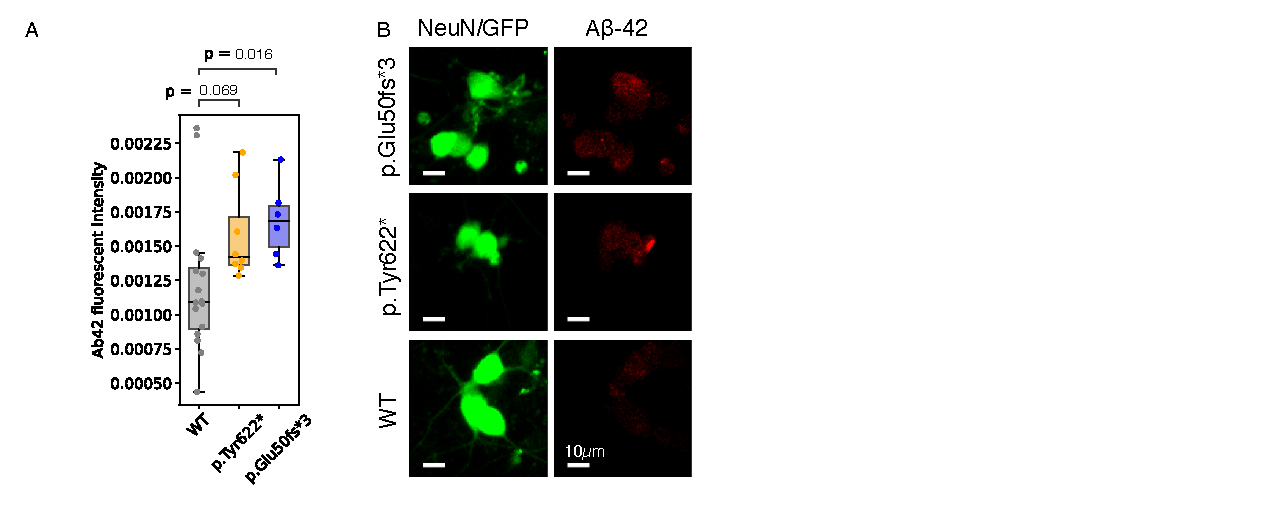
\includegraphics[width=\textwidth]{./extended_plots/quantification_Abeta42_iPSC_neurons.pdf}}
    \caption{
        \textbf{Quantification of Aβ42 in iPSC-Derived Neurons Harboring ABCA7 PTC Variants.}\\[1ex]
        (A) Quantification of neuronal Aβ42 fluorescence intensity. P-values were computed by a linear mixed-effects model on per-NeuN+ volume averages, including well-of-origin as a random effect. $N = 16$ (WT; 2261 cells), $N=8$ (p.Tyr622*; 1466 cells), $N=6$ wells (p.Glu50fs*3; 999 cells) from 4-week-old iNs. Boxes indicate per-condition dataset quartiles, and whiskers extend to the most extreme data points not considered outliers (i.e., within 1.5 times the interquartile range from the first or third quartile). Individual data points represent per-well averages of cell-level intensities. 
        (B) Representative images per condition showing mean-intensity projections of the entire image (NeuN+) and projections within NeuN+ volumes considered for quantification (Aβ42). Representative images for the Aβ42 channel were processed with condition-wide percentile-based background subtraction and thresholding. Representative images of cell soma underwent per-image percentile-based background subtraction and thresholding, reflecting the segmentation methodology.
    }
    \label{fig:quantification_Abeta42_iPSC_neurons}
\end{figure}

\begin{figure}[ht]
   % \centerline{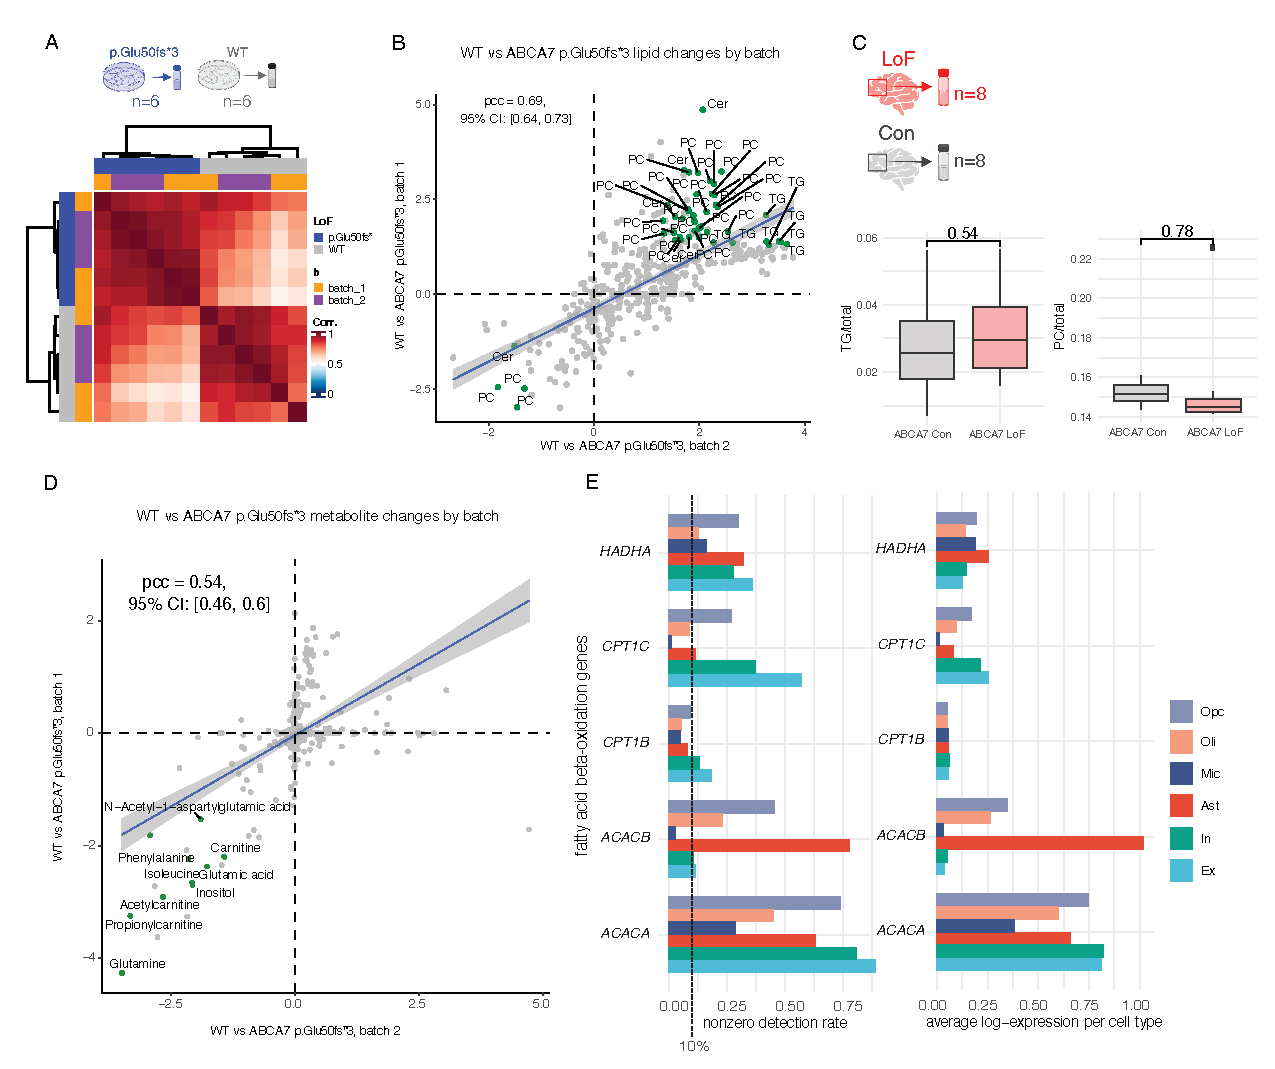
\includegraphics[width=\textwidth]{./extended_plots/lipidomic_analysis_iPSC_neurons.pdf}}
    \caption{
        \textbf{Lipidomic Analysis in ABCA7 LoF vs. Control iNs.}\\[1ex]
        (A) Pairwise Pearson correlation of iN lipidomic profiles. 
        (B) Correlation of lipidomic scores ($S = \text{sign}(\log(\text{fold-change})) \times -\log_{10}(\text{p-value})$, T-test) between WT and ABCA7 p.Glu50fs*3 iNs by batch. Top consistent triglyceride (TG), phosphatidylcholine (PC), and ceramide (Cer) lipid changes, where $|S| > 1.3$ in both batches, shown in green. Grey error bar indicates 95\% confidence interval for simple linear model fit. 
        (C) Relative TG and PC abundances in post-mortem human brain. Boxes indicate per-condition dataset quartiles, and whiskers extend to the most extreme data points not considered outliers (i.e., within 1.5 times the interquartile range from the first or third quartile). 
        (D) Correlation of metabolomic scores (computed and plotted as in B) for both differentiation batches. 
        (E) Average expression and nonzero detection rate of select lipid oxidation genes in major cell types in the human brain, assessed by snRNA-seq of post-mortem PFC.
    }
    \label{fig:lipidomic_analysis_iPSC_neurons}
\end{figure}

\begin{figure}[H]
    \begin{subfigure}[t]{0.33\textwidth}
        \caption{}
        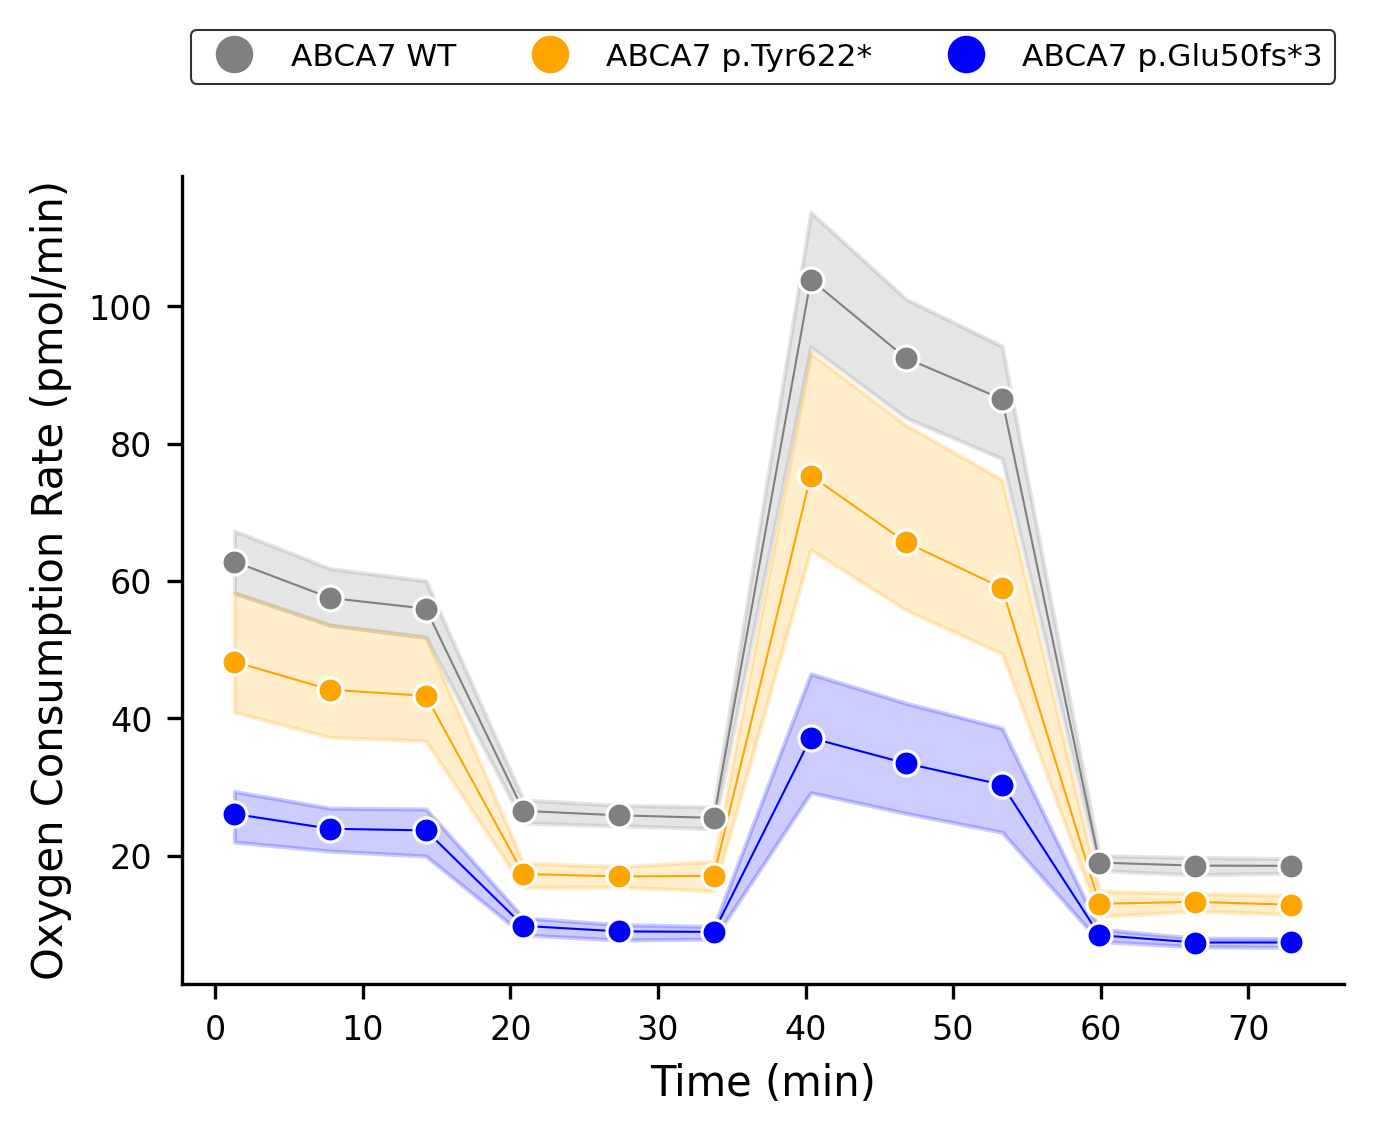
\includegraphics[width=\textwidth]{../paper/extended_plots/rep_seahorse_curves_by_line.png}        
    \end{subfigure}
    \begin{subfigure}[t]{0.33\textwidth}
        \caption{}
        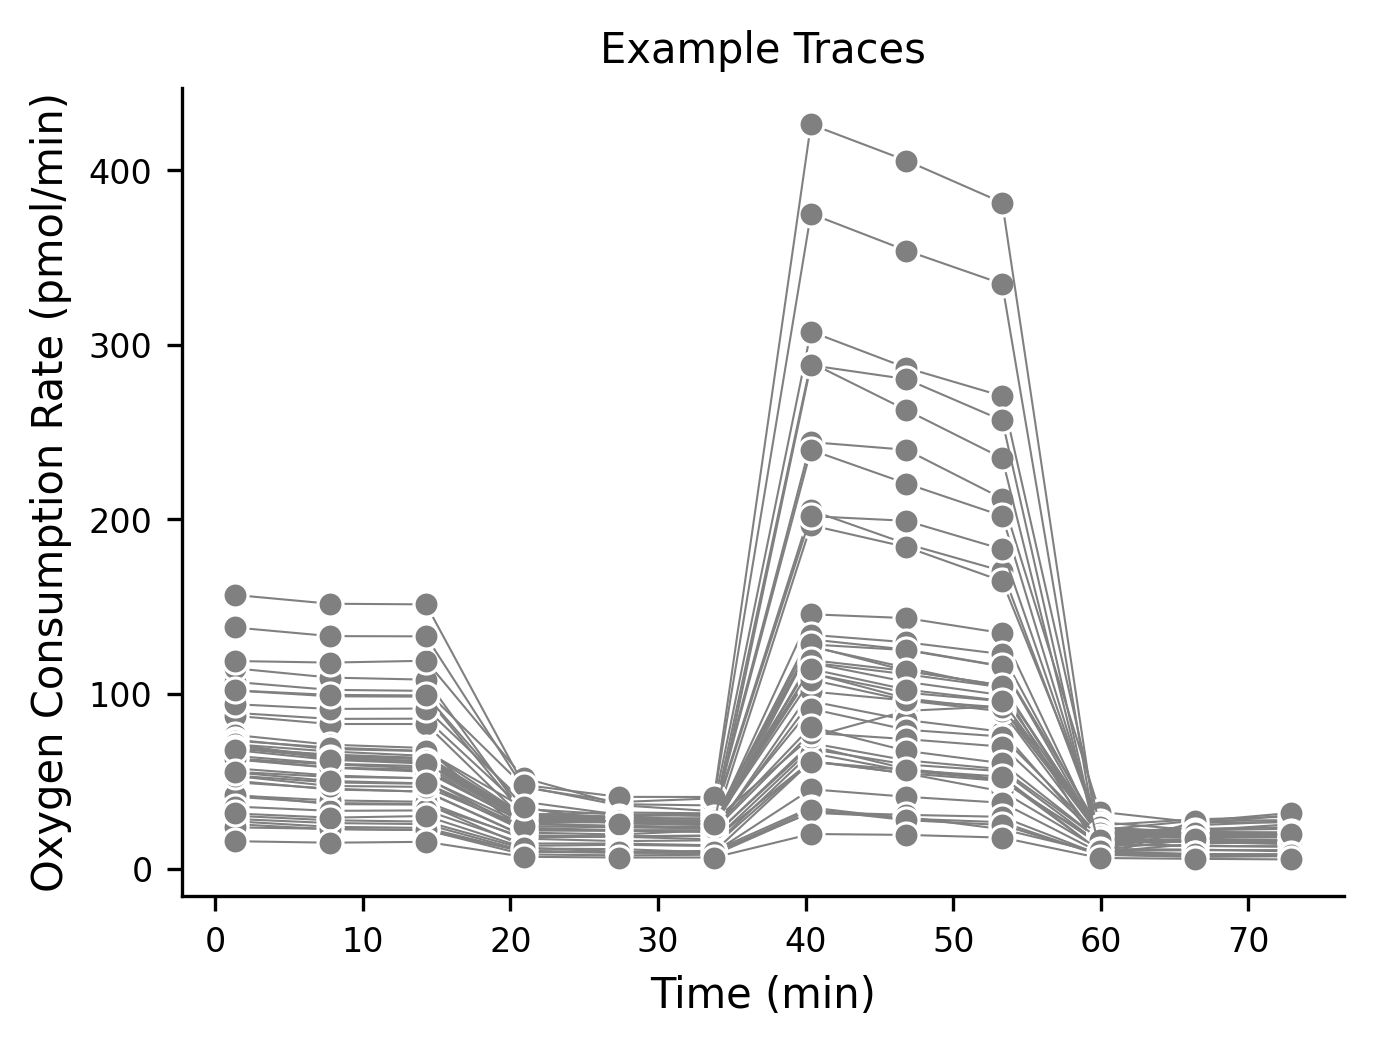
\includegraphics[width=\textwidth]{../paper/extended_plots/rep_seahorse_curves_all.png}        
    \end{subfigure}   
    \begin{subfigure}[t]{0.33\textwidth}
        \caption{}
        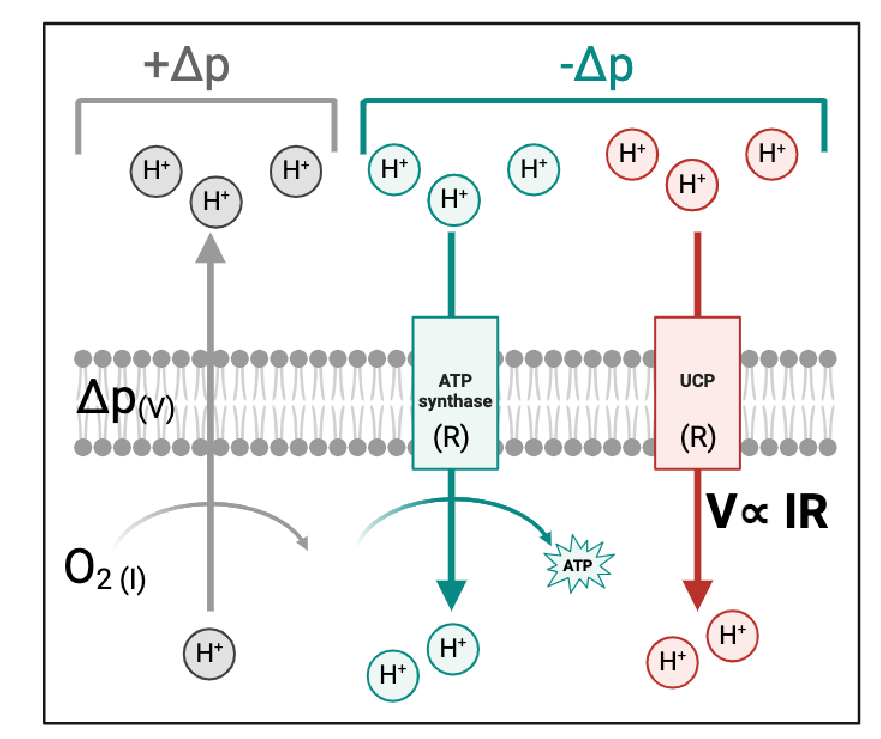
\includegraphics[width=\textwidth]{../paper/main_plots/uncoupling_cartoon.png}        
    \end{subfigure}  
    \begin{subfigure}[t]{0.33\textwidth}
        \caption{}
        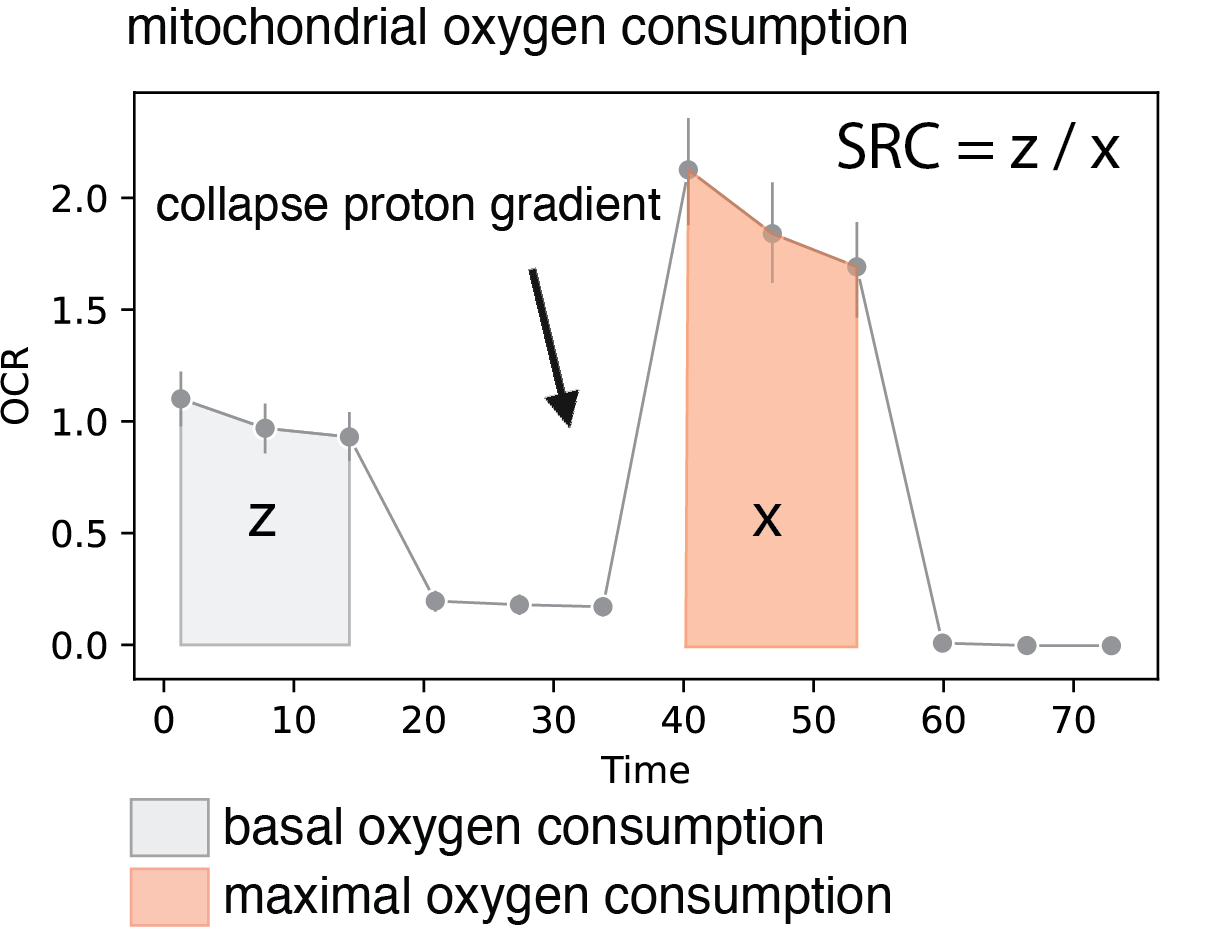
\includegraphics[width=\textwidth]{../paper/extended_plots/src_cartoon.png}        
    \end{subfigure} 
    \begin{subfigure}[t]{0.25\textwidth}
        \caption{}
        \includegraphics[width=\textwidth]{../paper/extended_plots/SRC.png}        
    \end{subfigure} 
    \begin{subfigure}[t]{0.33\textwidth}
        \caption{}
        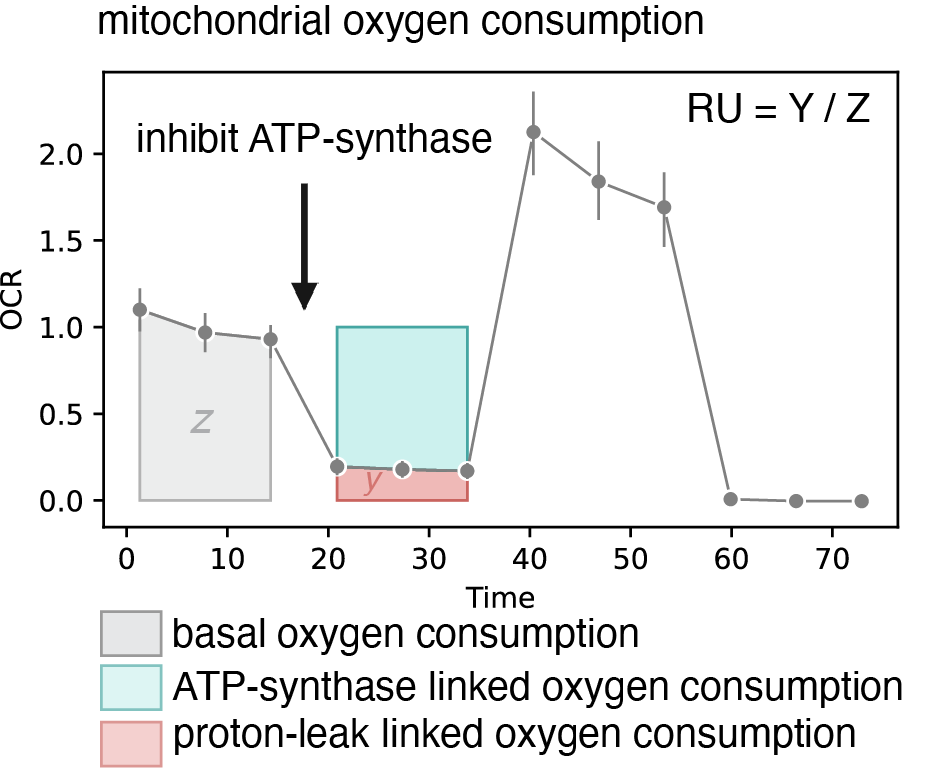
\includegraphics[width=\textwidth]{../paper/main_plots/seahorse_cartoon.png}        
    \end{subfigure}  
    \hspace{1cm}
    \begin{subfigure}[t]{0.3\textwidth}
        \caption{}
        \includegraphics[width=\textwidth]{../paper/extended_plots/UCP_levels.png}        
    \end{subfigure} 
    \par
    \centering
    \begin{subfigure}[t]{0.65\textwidth}
        \caption{}
        \includegraphics[width=\textwidth]{../paper/main_plots/tmrm_with_FCCP.png}        
    \end{subfigure} 
 \end{figure}
\textbf{Extended Data Fig. 10}
\clearpage

\begin{figure}[ht]
    \begin{subfigure}[t]{0.7\textwidth}
        \caption{}
        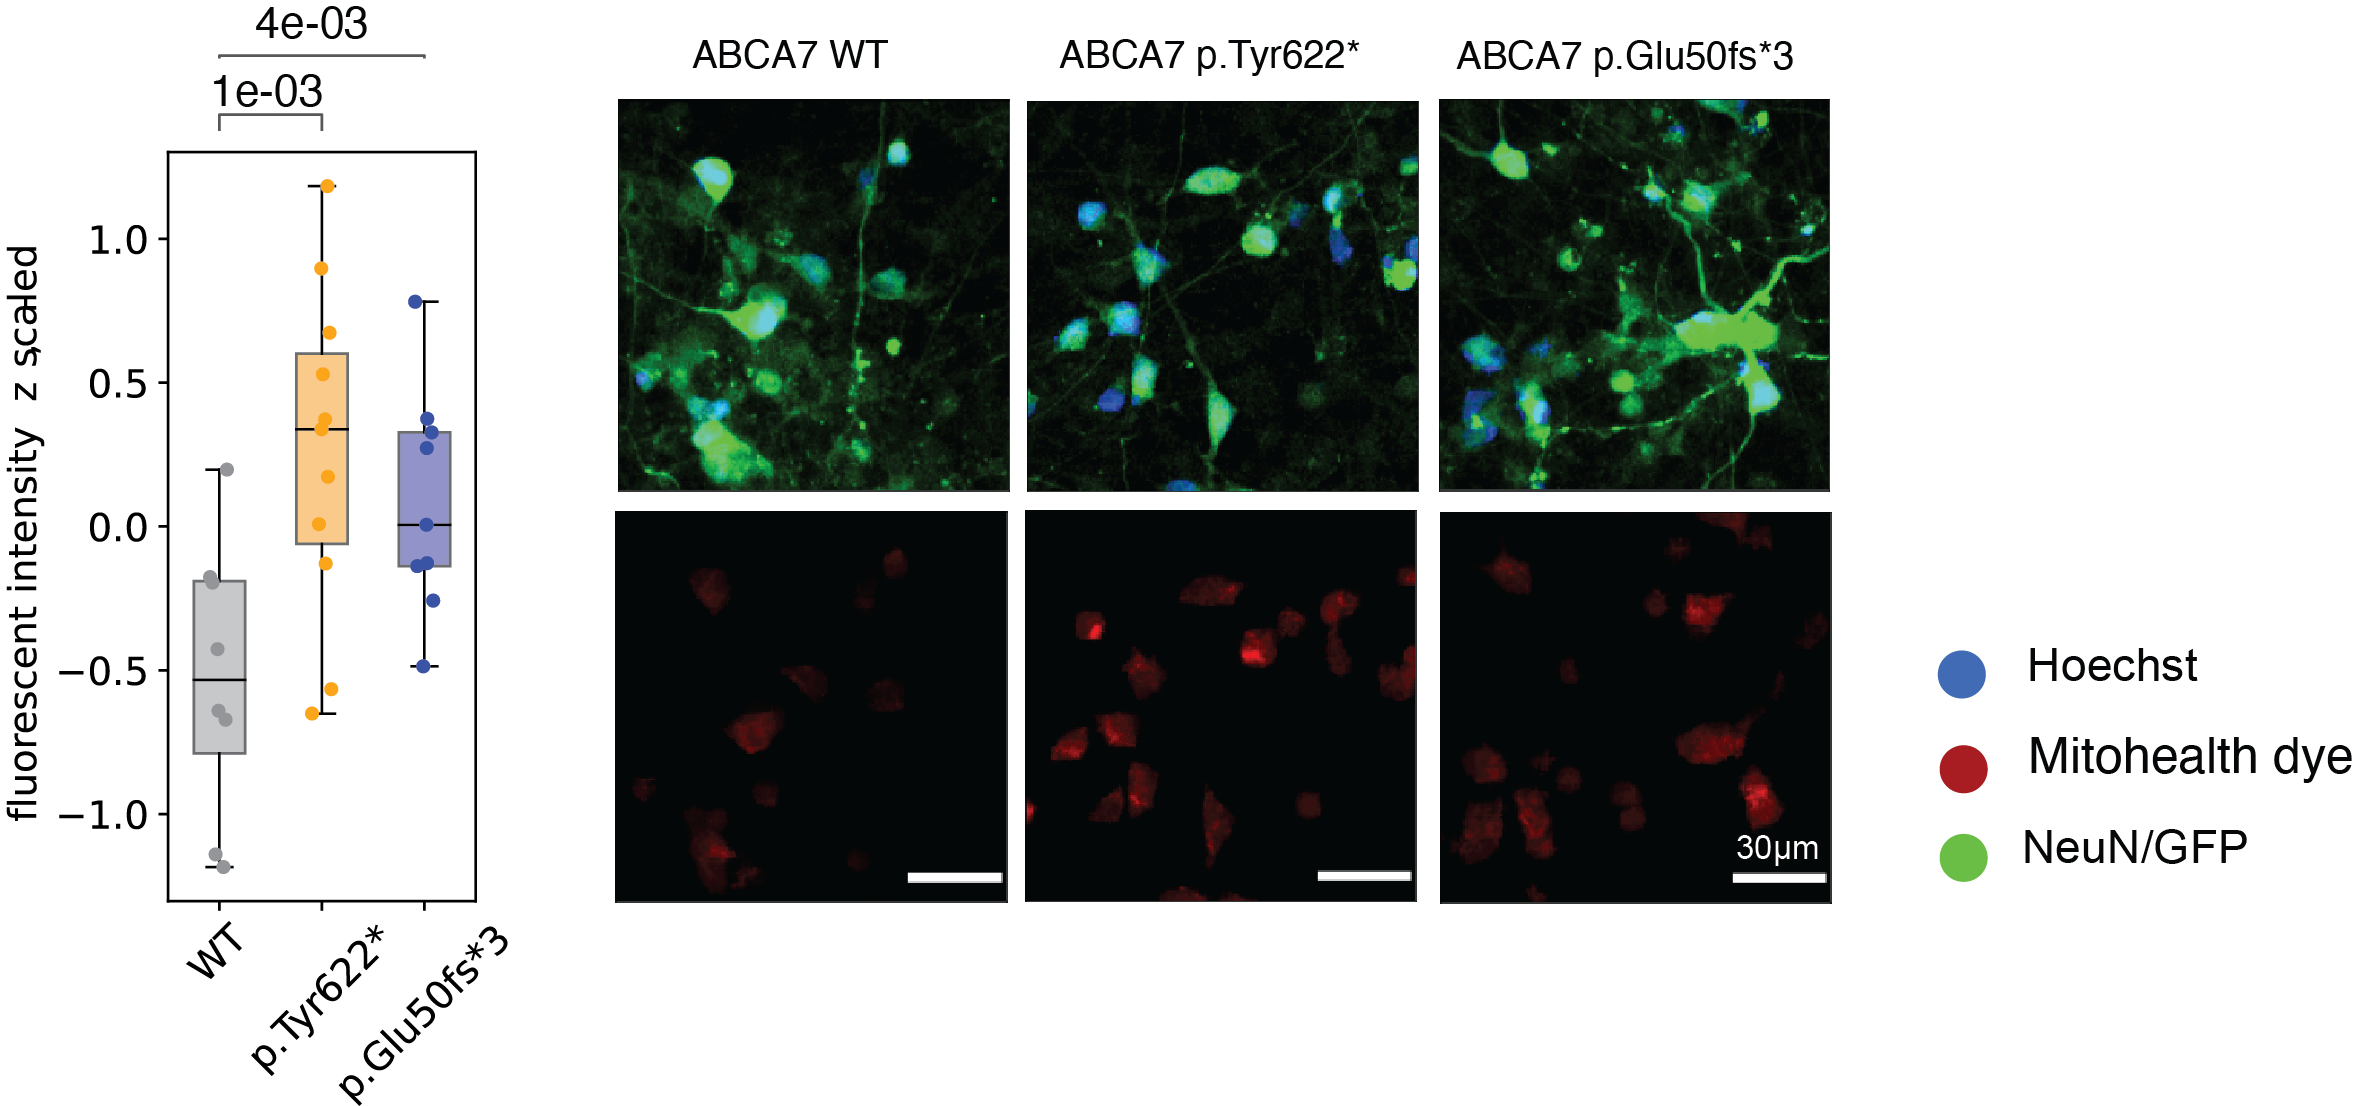
\includegraphics[width=\textwidth]{./extended_plots/mitohealth_dye.png}        
    \end{subfigure}
    \par
    \begin{subfigure}[t]{\textwidth}
        \caption{}
        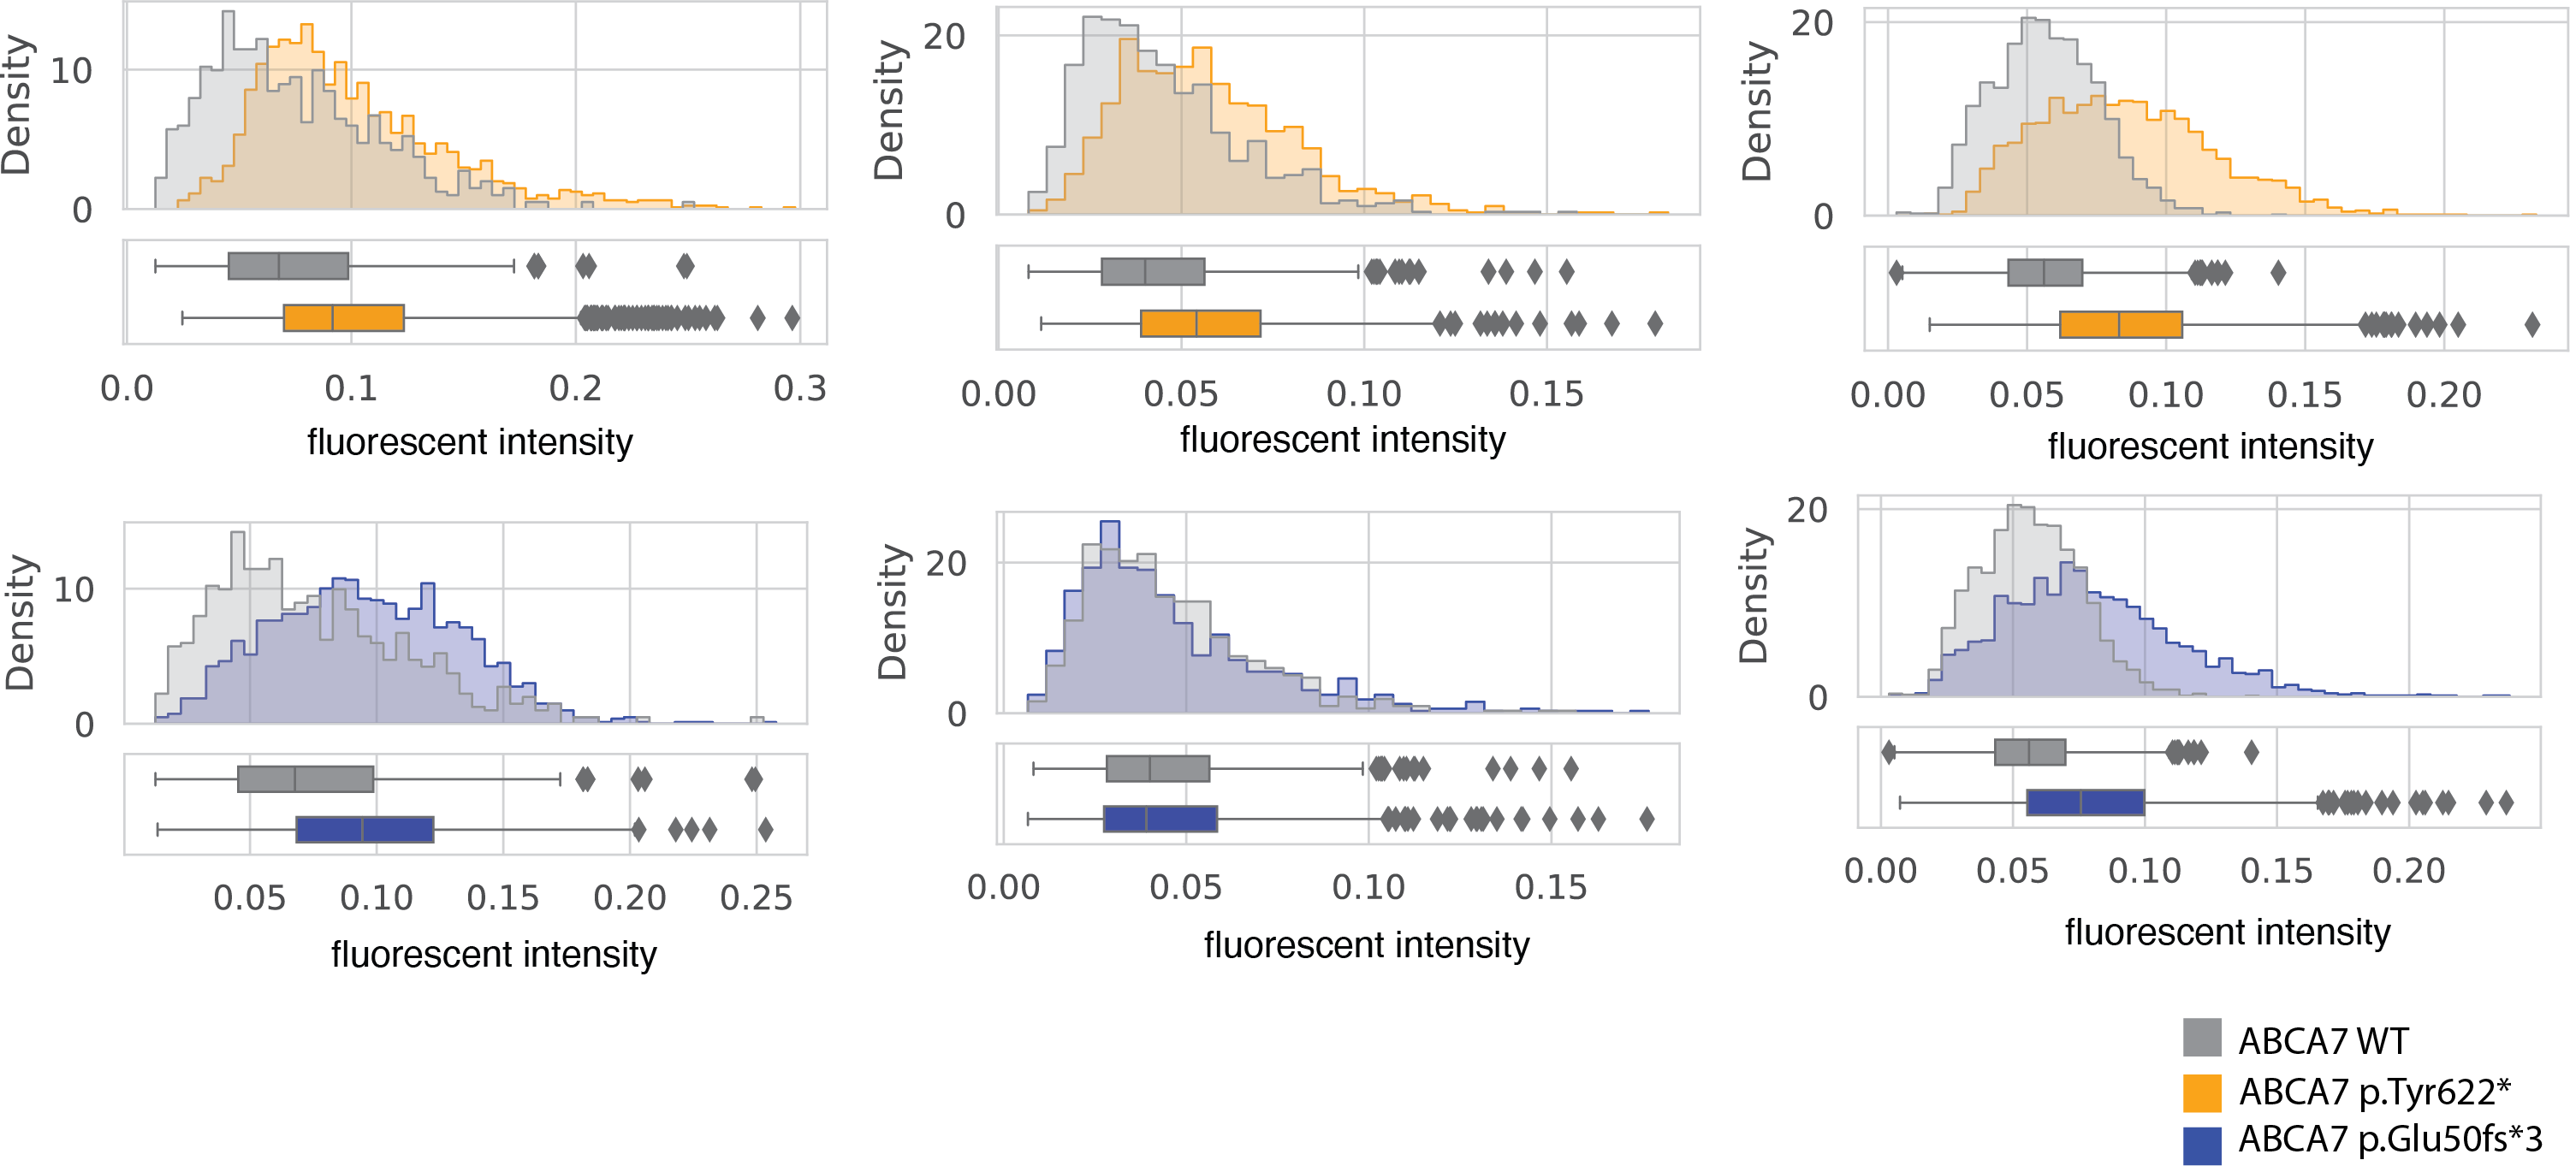
\includegraphics[width=\textwidth]{./extended_plots/mitohealth_per_cell.png}        
    \end{subfigure}
    \caption{
         \textbf{Analysis of Oxygen Consumption Rates in ABCA7 LoF vs. Control iNs.}\\[1ex]
         (A) Example oxygen consumption rate (OCR) curves from Batch 1 of the two differentiation batches used for analysis in Figure~\ref{fig:main_mitochondrial}G. The line plot indicates the per-condition mean estimator, and the error bars indicate the 95\% confidence interval. 
         (B) Representative per-well traces from (A). 
         (C) Schematic indicating measurement of maximal and basal oxygen consumption to compute SRC, as shown in 
         (D) for WT, ABCA7 p.Glu50fs*3, and ABCA7 p.Tyr622* iNs. P-values computed by independent sample t-test. $N$ wells = 18 (WT), 17 (p.Tyr622*), 13 (p.Glu50fs*3) across two independent differentiation batches and Seahorse experiments. 
         (E) Relative uncoupling measured for two independent iN differentiation batches and separate Seahorse experiments shown combined in Figure~\ref{fig:main_mitochondrial}G. P-values computed by independent sample t-test. Batch 1 (left); $N$ wells = 10 (WT), 7 (p.Tyr622*), 7 (p.Glu50fs*3). Batch 2 (right); $N$ wells = 8 (WT), 10 (p.Tyr622*), 6 (p.Glu50fs*3) shown per differentiation batch. For (D, E) boxes indicate per-condition dataset quartiles, and whiskers extend to the most extreme data points not considered outliers (i.e., within 1.5 times the interquartile range from the first or third quartile). 
         (F) Per-batch cell-level MioHealth fluorescence intensities (related to Figure~\ref{fig:main_mitochondrial}H).
     }
     \label{fig:oxygen_consumption_rates_iPSC_neurons}
 \end{figure}
\clearpage

\begin{figure}[ht]
   % \centerline{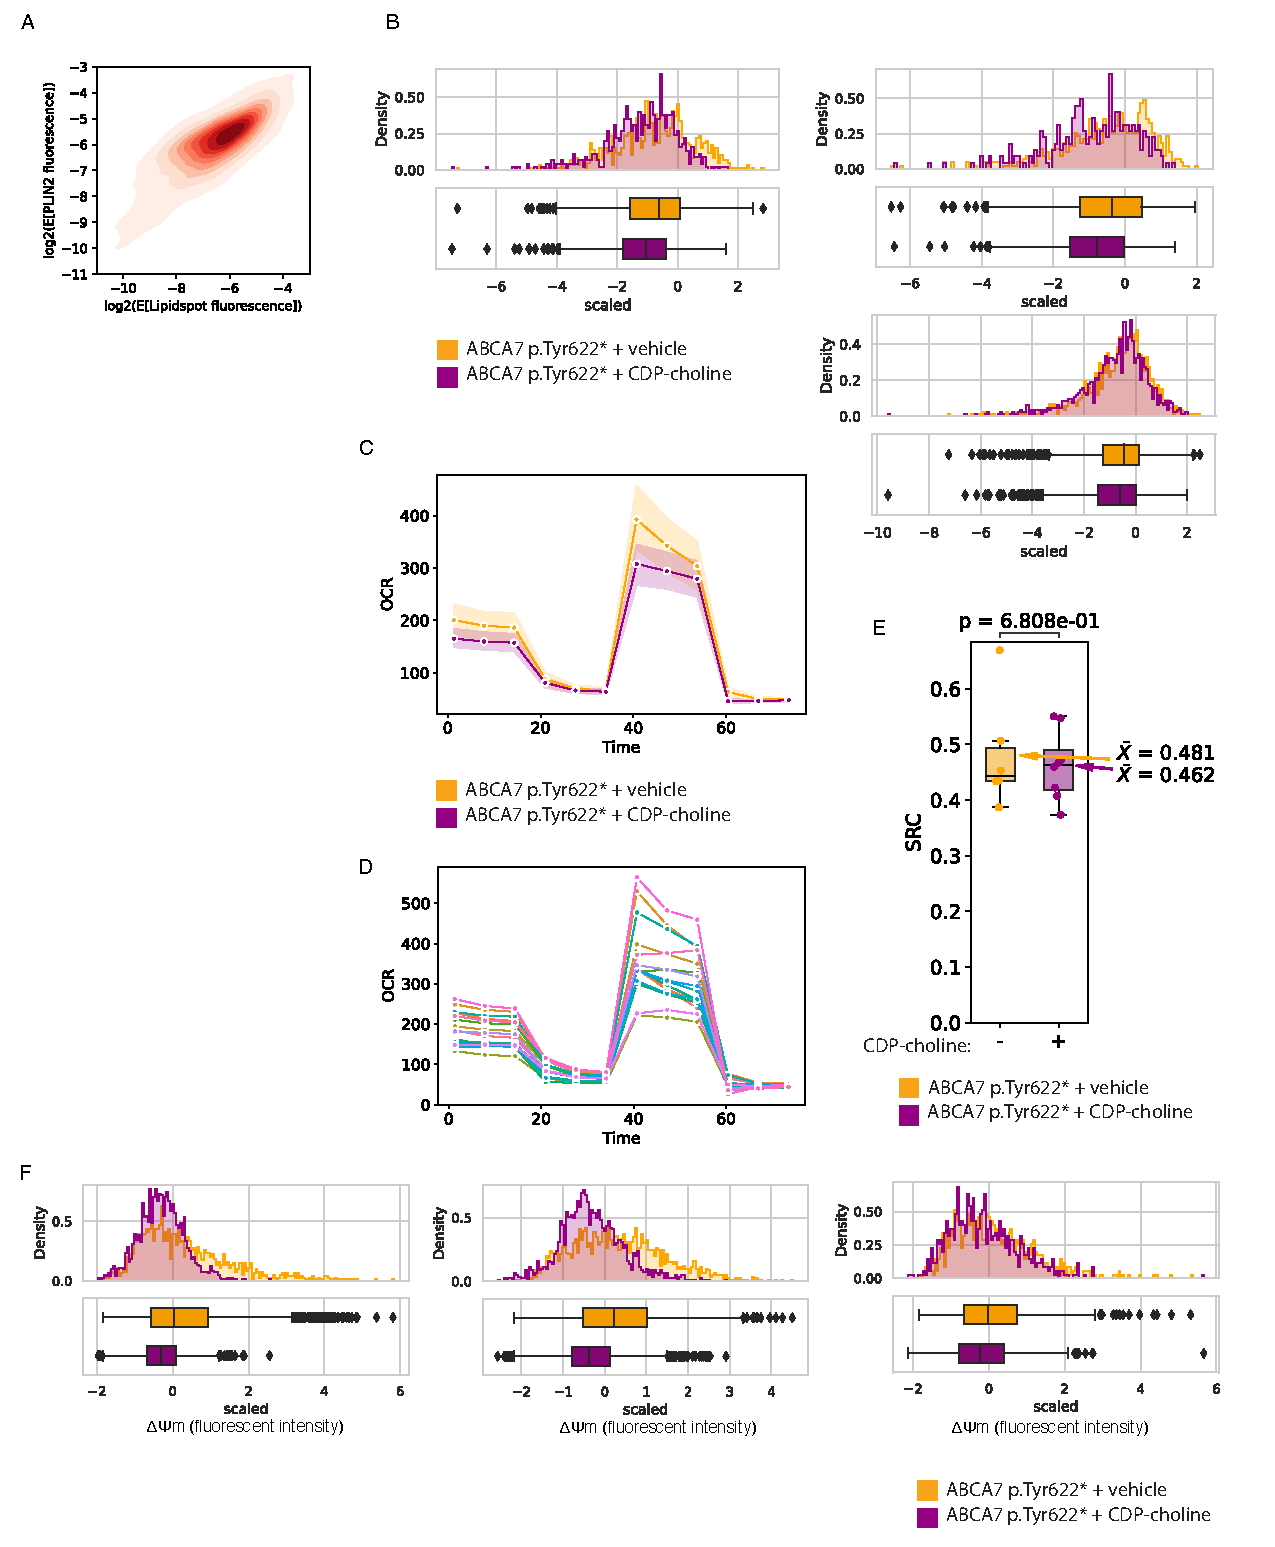
\includegraphics[width=\textwidth]{./extended_plots/lipid_mitochondrial_effects_CDP_choline.pdf}}
    \caption{
        \textbf{Lipid and Mitochondrial Effects of Treatment with CDP-choline.}\\[1ex]
        (A) Per-cell correlation of average PLIN2 and LipidSpot fluorescent intensities shown as a density plot. 
        (B) Per-batch LipidSpot fluorescence intensities (related to Figure~\ref{fig:main_choline}A) in ABCA7 p.Tyr622* iNs treated with CDP-choline or H20 vehicle control. X-axis indicates z-scaled log-fluorescence intensity. 
        (C) Example oxygen consumption rate (OCR) curves used for analysis in Figure~\ref{fig:main_choline}. The line plot indicates the per-condition mean estimator, and the error bars indicate the 95\% confidence interval. 
        (D) Representative per-well traces from (C). 
        (E) Quantification of SRC from curves in (D). P-values computed by independent sample t-test. $N$ wells = 6 (p.Tyr622* + H20), 8 (p.Tyr622* + CDP-choline). Boxes indicate per-condition dataset quartiles, and whiskers extend to the most extreme data points not considered outliers (i.e., within 1.5 times the interquartile range from the first or third quartile). 
        (F) Per-batch cell-level MioHealth fluorescence intensities (related to Figure~\ref{fig:main_choline}C) in ABCA7 p.Tyr622* iNs treated with CDP-choline or H20 vehicle control. X-axis indicates z-scaled fluorescence intensity.
    }
    \label{fig:lipid_mitochondrial_effects_CDP_choline}
\end{figure}
